% !TEX program = xelatex
% !TEX encoding = UTF-8
% ============================================
% 高中生物学常见遗传问题研究
% 基于数学笔记模板
% ============================================

\documentclass[a4paper, 11pt]{ctexart}

% ============================================
% 包的引入
% ============================================

% 数学公式与符号
\usepackage{amsmath, amssymb, amsthm, amsfonts}
\usepackage{mathtools} % 增强的数学工具

% 页面设置
\usepackage{geometry}
\geometry{left=2cm, right=2cm, top=2.5cm, bottom=2.5cm}

% 颜色支持
\usepackage{xcolor}

% 绘图支持
\usepackage{tikz}
\usetikzlibrary{arrows.meta, positioning, intersections, quotes, calc, shapes.geometric, matrix}

% 彩色文本框
\usepackage[most]{tcolorbox}

% 超链接
\usepackage[colorlinks=true, linkcolor=myblue, citecolor=mygreen, urlcolor=myred]{hyperref}

% 图片支持
\usepackage{graphicx}

% 其他工具
\usepackage{caption} % 支持 \captionof 命令
\usepackage{enumitem} % 增强的列表环境
\usepackage{multirow} % 表格多行合并
\usepackage{array} % 表格列格式

% ============================================
% 颜色定义(兼容黑白打印)
% ============================================
\definecolor{myblue}{RGB}{0, 112, 192}
\definecolor{mygreen}{RGB}{0, 176, 80}
\definecolor{myorange}{RGB}{247, 150, 70}
\definecolor{myred}{RGB}{200, 0, 0}
\definecolor{mypurple}{RGB}{152, 78, 163}
\definecolor{mygray}{gray}{0.95}

% ============================================
% 定理、定义、例题环境设置
% ============================================

% 定理环境
\newtcolorbox{theorembox}[1]{
    colback=myblue!5!white,
    colframe=myblue!75!black,
    fonttitle=\bfseries,
    title=遗传定律:#1,
    enhanced,
    attach boxed title to top left={xshift=1cm, yshift=-2mm},
    top=8mm,
    boxed title style={
        colback=myblue!75!black,
        sharp corners
    }
}

% 定义环境
\newtcolorbox{definitionbox}[1]{
    colback=mygreen!5!white,
    colframe=mygreen!75!black,
    fonttitle=\bfseries,
    title=定义:#1,
    enhanced,
    attach boxed title to top left={xshift=1cm, yshift=-2mm},
    top=8mm,
    boxed title style={
        colback=mygreen!75!black,
        sharp corners
    }
}

% 例题/技巧与应用环境
\newtcolorbox{examplebox}[1]{
    colback=myorange!5!white,
    colframe=myorange!75!black,
    fonttitle=\bfseries,
    title=解题技巧:#1,
    enhanced,
    attach boxed title to top left={xshift=1cm, yshift=-2mm},
    top=8mm,
    boxed title style={
        colback=myorange!75!black,
        sharp corners
    }
}

% 引理环境
\newtcolorbox{lemmabox}[1]{
    colback=mypurple!5!white,
    colframe=mypurple!75!black,
    fonttitle=\bfseries,
    title=关键要点:#1,
    enhanced,
    attach boxed title to top left={xshift=1cm, yshift=-2mm},
    top=8mm,
    boxed title style={
        colback=mypurple!75!black,
        sharp corners
    }
}

% 注意/提醒环境
\newtcolorbox{notebox}[1]{
    colback=mygray,
    colframe=myred!75!black,
    fonttitle=\bfseries,
    title=注意事项:#1,
    enhanced,
    attach boxed title to top left={xshift=1cm, yshift=-2mm},
    top=8mm,
    boxed title style={
        colback=myred!75!black,
        sharp corners
    }
}

% ============================================
% 标题格式设置
% ============================================
\usepackage{titlesec}
\titleformat{\section}
    {\Large\bfseries\color{myblue}}
    {\thesection}{1em}{}
\titleformat{\subsection}
    {\large\bfseries\color{myorange}}
    {\thesubsection}{1em}{}

% ============================================
% 数学定理环境(使用 amsthm)
% ============================================
\theoremstyle{definition}
\newtheorem{theorem}{定律}[section]
\newtheorem{definition}{定义}[section]
\newtheorem{lemma}{引理}[section]
\newtheorem{corollary}{推论}[theorem]
\newtheorem{example}{例题}[section]

% ============================================
% 自定义命令
% ============================================
\newcommand{\genotype}[1]{\textcolor{myblue}{\textbf{#1}}} % 基因型
\newcommand{\phenotype}[1]{\textcolor{myred}{\textbf{#1}}} % 表现型

% ============================================
% 文档开始
% ============================================
\begin{document}

% 标题页
\title{\Huge \bfseries \color{myblue} 高中生物学常见遗传问题研究}
\author{生物学笔记}
\date{\today}
\maketitle

% 目录
\tableofcontents
\newpage

% ============================================
% 第一部分:基础概念
% ============================================

\section{第一部分:遗传学基础概念}

\subsection{核心术语}

\begin{definitionbox}{等位基因}
\textbf{等位基因}(allele):控制相对性状的成对基因,位于同源染色体的相同位置上。

例如:控制豌豆高茎和矮茎的基因 $A$ 和 $a$ 就是一对等位基因。
\end{definitionbox}

\begin{definitionbox}{基因型与表现型}
\textbf{基因型}(genotype):生物个体基因的组成,如 $AA$、$Aa$、$aa$。

\textbf{表现型}(phenotype):生物个体表现出来的性状,如高茎、矮茎。

\textbf{关系}:表现型 = 基因型 + 环境条件
\end{definitionbox}

\begin{definitionbox}{纯合子与杂合子}
\textbf{纯合子}(homozygote):基因型中成对的等位基因相同,如 $AA$、$aa$。

\textbf{杂合子}(heterozygote):基因型中成对的等位基因不同,如 $Aa$。
\end{definitionbox}

\begin{definitionbox}{显性与隐性}
\textbf{显性基因}:在杂合子中能表现出其性状的基因,用大写字母表示(如 $A$)。

\textbf{隐性基因}:在杂合子中不能表现出其性状的基因,用小写字母表示(如 $a$)。

\textbf{显性性状}:由显性基因控制的性状。

\textbf{隐性性状}:只有在隐性纯合子中才能表现出来的性状。
\end{definitionbox}

\subsection{遗传符号系统}

\begin{lemmabox}{常用符号约定}
\begin{itemize}[leftmargin=2em]
    \item 显性基因:大写字母($A$、$B$、$D$ 等)
    \item 隐性基因:小写字母($a$、$b$、$d$ 等)
    \item 父本:$\mathcal{P}$ 或 P(父本)
    \item 母本:$\mathcal{P}$ 或 P(母本)
    \item 子一代:$F_1$
    \item 子二代:$F_2$
    \item 杂交:$\times$
    \item 自交:$\bigcirc$
\end{itemize}
\end{lemmabox}

% ============================================
% 第二部分:孟德尔遗传定律
% ============================================

\section{第二部分:孟德尔遗传定律}

\subsection{分离定律}

\begin{theorembox}{分离定律(Law of Segregation)}
在生物的体细胞中,控制同一性状的遗传因子成对存在,不相融合;在形成配子时,成对的遗传因子发生分离,分离后的遗传因子分别进入不同的配子中,随配子遗传给后代。

\textbf{核心要点}:
\begin{enumerate}[leftmargin=2em]
    \item 成对的等位基因在形成配子时分离
    \item 分离后的基因独立进入不同的配子
    \item 配子中只含等位基因中的一个
\end{enumerate}
\end{theorembox}

\begin{examplebox}{分离定律的验证}
\textbf{实验}:$F_1$ 高茎豌豆($Aa$)自交

\textbf{过程}:
\begin{enumerate}[leftmargin=2em]
    \item $F_1$ 产生配子:$A$ 和 $a$,比例 $1:1$
    \item 雌雄配子随机结合
    \item $F_2$ 基因型:$AA : Aa : aa = 1 : 2 : 1$
    \item $F_2$ 表现型:高茎 : 矮茎 = $3 : 1$
\end{enumerate}

\begin{center}
\begin{tikzpicture}[scale=0.9]
    % 父本
    \node[rectangle, draw=myblue, thick, minimum width=2cm, minimum height=0.8cm] (P) at (0, 4) {$F_1: Aa$};
    \node[below=0.2cm of P] {高茎};
    
    % 配子
    \node[circle, draw=mygreen, thick, minimum size=0.8cm] (g1) at (-1.5, 2.5) {$A$};
    \node[circle, draw=mygreen, thick, minimum size=0.8cm] (g2) at (1.5, 2.5) {$a$};
    \draw[->, mygreen, thick] (P) -- (g1);
    \draw[->, mygreen, thick] (P) -- (g2);
    \node[below=0.1cm of g1] {$\frac{1}{2}$};
    \node[below=0.1cm of g2] {$\frac{1}{2}$};
    
    % 配子结合
    \node[below=0.5cm of g1, font=\small] {雄配子};
    \node[below=0.5cm of g2, font=\small] {雄配子};
    
    % 棋盘格
    \node[circle, draw=mygreen, thick, minimum size=0.6cm] (fg1) at (-1.5, 1) {$A$};
    \node[circle, draw=mygreen, thick, minimum size=0.6cm] (fg2) at (1.5, 1) {$a$};
    \node[left=0.3cm of fg1, font=\small] {雌};
    \node[left=0.3cm of fg2, font=\small] {配};
    
    % F2结果
    \node[rectangle, draw=myorange, thick, minimum width=1.2cm, minimum height=0.6cm] (f1) at (-1.5, -0.5) {$AA$};
    \node[rectangle, draw=myorange, thick, minimum width=1.2cm, minimum height=0.6cm] (f2) at (0, -0.5) {$Aa$};
    \node[rectangle, draw=myorange, thick, minimum width=1.2cm, minimum height=0.6cm] (f3) at (1.5, -0.5) {$Aa$};
    \node[rectangle, draw=myorange, thick, minimum width=1.2cm, minimum height=0.6cm] (f4) at (0, -1.2) {$aa$};
    
    \draw[->, mypurple] (fg1) -- (f1);
    \draw[->, mypurple] (fg1) -- (f2);
    \draw[->, mypurple] (fg2) -- (f3);
    \draw[->, mypurple] (fg2) -- (f4);
    
    \node[below=0.2cm of f1, font=\tiny] {高};
    \node[below=0.2cm of f2, font=\tiny] {高};
    \node[below=0.2cm of f3, font=\tiny] {高};
    \node[below=0.2cm of f4, font=\tiny] {矮};
    
    \node[below=1cm of f2] {$F_2$ 表现型比例:高茎 : 矮茎 = $3 : 1$};
\end{tikzpicture}
\captionof{figure}{分离定律图解}
\end{center}
\end{examplebox}

\subsection{自由组合定律}

\begin{theorembox}{自由组合定律(Law of Independent Assortment)}
控制不同性状的遗传因子的分离和组合是互不干扰的;在形成配子时,决定同一性状的成对的遗传因子彼此分离,决定不同性状的遗传因子自由组合。

\textbf{适用条件}:
\begin{enumerate}[leftmargin=2em]
    \item 两对或两对以上的等位基因
    \item 控制不同性状的基因位于非同源染色体上
    \item 各对基因独立遗传
\end{enumerate}
\end{theorembox}

\begin{examplebox}{自由组合定律的验证}
\textbf{实验}:黄色圆粒($YYRR$)$\times$ 绿色皱粒($yyrr$)

\textbf{$F_1$}:黄色圆粒($YyRr$)

\textbf{$F_1$ 自交产生 $F_2$}:

$F_1$ 产生配子类型:$YR$、$Yr$、$yR$、$yr$,比例 $1:1:1:1$

\begin{center}
\begin{tikzpicture}[scale=0.75]
    \matrix[matrix of nodes, 
            nodes={draw, minimum width=1.2cm, minimum height=0.6cm, anchor=center},
            column sep=0.1cm, row sep=0.1cm,
            ampersand replacement=\&] (m) {
        \& $YR$ \& $Yr$ \& $yR$ \& $yr$ \\
        $YR$ \& $YYRR$ \& $YYRr$ \& $YyRR$ \& $YyRr$ \\
        $Yr$ \& $YYRr$ \& $YYrr$ \& $YyRr$ \& $Yyrr$ \\
        $yR$ \& $YyRR$ \& $YyRr$ \& $yyRR$ \& $yyRr$ \\
        $yr$ \& $YyRr$ \& $Yyrr$ \& $yyRr$ \& $yyrr$ \\
    };
    
    % 第一行和第一列样式
    \foreach \i in {2,3,4,5} {
        \node[fill=mygreen!30, font=\small] at (m-1-\i) {};
        \node[fill=mygreen!30, font=\small] at (m-\i-1) {};
    }
    
    % 标注
    \node[left=0.3cm of m-2-1, font=\small] {雌配子};
    \node[above=0.1cm of m-1-2, font=\small, xshift=-0.5cm] {雄配子};
    
    % 表现型标注(简化)
    \node[below=0.8cm of m-5-3, font=\small] {$F_2$ 表现型:};
    \node[below=1.2cm of m-5-2, font=\tiny, align=center] {黄圆\\9};
    \node[below=1.2cm of m-5-3, font=\tiny, align=center] {黄皱\\3};
    \node[below=1.2cm of m-5-4, font=\tiny, align=center] {绿圆\\3};
    \node[below=1.2cm of m-5-5, font=\tiny, align=center] {绿皱\\1};
\end{tikzpicture}
\captionof{figure}{自由组合定律棋盘格($F_2$)}
\end{center}

\textbf{$F_2$ 表现型比例}:黄色圆粒 : 黄色皱粒 : 绿色圆粒 : 绿色皱粒 = $9:3:3:1$

\textbf{$F_2$ 基因型种类}:$3^2 = 9$ 种
\end{examplebox}

% ============================================
% 第三部分:配子法
% ============================================

\section{第三部分:配子法(核心方法)}

\subsection{配子法的基本原理}

\begin{definitionbox}{配子法}
\textbf{配子法}是通过分析亲本产生配子的类型和比例,然后计算配子随机结合后子代基因型和表现型的方法。

\textbf{核心步骤}:
\begin{enumerate}[leftmargin=2em]
    \item 确定亲本基因型
    \item 分析亲本产生的配子类型及比例
    \item 计算配子结合的概率
    \item 统计子代基因型和表现型
\end{enumerate}
\end{definitionbox}

\begin{lemmabox}{配子产生的规律}
\begin{itemize}[leftmargin=2em]
    \item \textbf{一对等位基因}:$Aa$ 产生 $A$ 和 $a$,比例 $1:1$
    \item \textbf{两对等位基因}(独立遗传):
        \begin{itemize}
            \item $AaBb$ 产生 $AB$、$Ab$、$aB$、$ab$,比例 $1:1:1:1$
            \item 配子种类数 = $2^n$($n$ 为杂合基因对数)
        \end{itemize}
    \item \textbf{多对等位基因}:每对基因独立分离,然后自由组合
\end{itemize}
\end{lemmabox}

\subsection{一对相对性状的配子法}

\begin{examplebox}{基础配子法应用}
\textbf{题目}:高茎豌豆($Aa$)与矮茎豌豆($aa$)杂交,求子代基因型和表现型。

\textbf{解题步骤}:

\textbf{步骤 1}:确定亲本基因型
\begin{itemize}[leftmargin=2em]
    \item 亲本 1:$Aa$(高茎)
    \item 亲本 2:$aa$(矮茎)
\end{itemize}

\textbf{步骤 2}:分析配子类型及比例
\begin{itemize}[leftmargin=2em]
    \item $Aa$ 产生:$A$ ($\frac{1}{2}$)、$a$ ($\frac{1}{2}$)
    \item $aa$ 产生:$a$ ($1$)
\end{itemize}

\textbf{步骤 3}:配子结合(利用概率)
\begin{itemize}[leftmargin=2em]
    \item $Aa$ 的概率:$P(A) \times P(a) = \frac{1}{2} \times 1 = \frac{1}{2}$
    \item $aa$ 的概率:$P(a) \times P(a) = \frac{1}{2} \times 1 = \frac{1}{2}$
\end{itemize}

\textbf{步骤 4}:结果
\begin{itemize}[leftmargin=2em]
    \item 基因型:$Aa : aa = 1 : 1$
    \item 表现型:高茎 : 矮茎 = $1 : 1$
\end{itemize}

\begin{center}
\begin{tikzpicture}[scale=0.9]
    % 亲本
    \node[rectangle, draw=myblue, thick, minimum width=2cm, minimum height=0.8cm] (P1) at (-2, 3) {$Aa$};
    \node[rectangle, draw=myblue, thick, minimum width=2cm, minimum height=0.8cm] (P2) at (2, 3) {$aa$};
    
    % 配子
    \node[circle, draw=mygreen, thick, minimum size=0.7cm] (g1) at (-2.5, 1.5) {$A$};
    \node[circle, draw=mygreen, thick, minimum size=0.7cm] (g2) at (-1.5, 1.5) {$a$};
    \node[circle, draw=mygreen, thick, minimum size=0.7cm] (g3) at (2, 1.5) {$a$};
    
    \draw[->, mygreen] (P1) -- (g1);
    \draw[->, mygreen] (P1) -- (g2);
    \draw[->, mygreen] (P2) -- (g3);
    
    \node[below=0.1cm of g1, font=\tiny] {$\frac{1}{2}$};
    \node[below=0.1cm of g2, font=\tiny] {$\frac{1}{2}$};
    \node[below=0.1cm of g3, font=\tiny] {$1$};
    
    % 结合
    \node[rectangle, draw=myorange, thick, minimum width=1.5cm, minimum height=0.6cm] (r1) at (-2, 0) {$Aa$};
    \node[rectangle, draw=myorange, thick, minimum width=1.5cm, minimum height=0.6cm] (r2) at (0.5, 0) {$aa$};
    
    \draw[->, mypurple] (g1) -- (r1);
    \draw[->, mypurple] (g2) -- (r2);
    \draw[->, mypurple] (g3) to[out=270, in=90] (r1);
    \draw[->, mypurple] (g3) to[out=270, in=90] (r2);
    
    \node[below=0.2cm of r1, font=\small] {高茎 $\frac{1}{2}$};
    \node[below=0.2cm of r2, font=\small] {矮茎 $\frac{1}{2}$};
\end{tikzpicture}
\captionof{figure}{一对相对性状配子法图解}
\end{center}
\end{examplebox}

\subsection{两对相对性状的配子法}

\begin{examplebox}{两对相对性状的配子法}
\textbf{题目}:$AaBb$ 与 $Aabb$ 杂交,求子代基因型和表现型。

\textbf{方法一:完整配子法}

\textbf{步骤 1}:确定配子类型及比例
\begin{itemize}[leftmargin=2em]
    \item $AaBb$ 产生:$AB$ ($\frac{1}{4}$)、$Ab$ ($\frac{1}{4}$)、$aB$ ($\frac{1}{4}$)、$ab$ ($\frac{1}{4}$)
    \item $Aabb$ 产生:$Ab$ ($\frac{1}{2}$)、$ab$ ($\frac{1}{2}$)
\end{itemize}

\textbf{步骤 2}:配子结合(棋盘格法)

\begin{center}
\begin{tabular}{|c|c|c|}
\hline
\multirow{2}{*}{$AaBb$ 配子} & \multicolumn{2}{c|}{$Aabb$ 配子} \\
\cline{2-3}
 & $Ab$ ($\frac{1}{2}$) & $ab$ ($\frac{1}{2}$) \\
\hline
$AB$ ($\frac{1}{4}$) & $AABb$ ($\frac{1}{8}$) & $AaBb$ ($\frac{1}{8}$) \\
\hline
$Ab$ ($\frac{1}{4}$) & $AAbb$ ($\frac{1}{8}$) & $Aabb$ ($\frac{1}{8}$) \\
\hline
$aB$ ($\frac{1}{4}$) & $AaBb$ ($\frac{1}{8}$) & $aaBb$ ($\frac{1}{8}$) \\
\hline
$ab$ ($\frac{1}{4}$) & $Aabb$ ($\frac{1}{8}$) & $aabb$ ($\frac{1}{8}$) \\
\hline
\end{tabular}
\end{center}

\textbf{步骤 3}:统计结果
\begin{itemize}[leftmargin=2em]
    \item \textbf{基因型}(合并相同):
        \begin{itemize}
            \item $AABb$: $\frac{1}{8}$
            \item $AaBb$: $\frac{1}{8} + \frac{1}{8} = \frac{2}{8} = \frac{1}{4}$
            \item $AAbb$: $\frac{1}{8}$
            \item $Aabb$: $\frac{1}{8} + \frac{1}{8} = \frac{2}{8} = \frac{1}{4}$
            \item $aaBb$: $\frac{1}{8}$
            \item $aabb$: $\frac{1}{8}$
        \end{itemize}
    \item \textbf{表现型}(假设 $A$、$B$ 为显性):
        \begin{itemize}
            \item $A\_B\_$: $\frac{1}{8} + \frac{2}{8} = \frac{3}{8}$
            \item $A\_bb$: $\frac{1}{8} + \frac{2}{8} = \frac{3}{8}$
            \item $aaB\_$: $\frac{1}{8}$
            \item $aabb$: $\frac{1}{8}$
        \end{itemize}
\end{itemize}

\textbf{方法二:分离定律分别计算}

将两对基因分别考虑,然后用乘法原理:

\textbf{第一对基因} ($Aa \times Aa$):
\begin{itemize}[leftmargin=2em]
    \item $AA$: $\frac{1}{4}$,$Aa$: $\frac{1}{2}$,$aa$: $\frac{1}{4}$
\end{itemize}

\textbf{第二对基因} ($Bb \times bb$):
\begin{itemize}[leftmargin=2em]
    \item $Bb$: $\frac{1}{2}$,$bb$: $\frac{1}{2}$
\end{itemize}

\textbf{组合}(乘法原理):
\begin{itemize}[leftmargin=2em]
    \item $AABb$: $\frac{1}{4} \times \frac{1}{2} = \frac{1}{8}$
    \item $AaBb$: $\frac{1}{2} \times \frac{1}{2} = \frac{1}{4}$
    \item 其他类似计算...
\end{itemize}

\textbf{优势}:方法二计算更快捷,适合复杂问题。
\end{examplebox}

\subsection{三对相对性状的配子法}

\begin{examplebox}{三对等位基因的配子法}
\textbf{题目}:$AaBbCc$ 自交,求 $F_2$ 的基因型种类、表现型种类及比例。

\textbf{解题}:

\textbf{方法:分离定律分别计算}

\textbf{第一对基因} ($Aa \times Aa$):
\begin{itemize}[leftmargin=2em]
    \item 基因型:$AA$ ($\frac{1}{4}$)、$Aa$ ($\frac{1}{2}$)、$aa$ ($\frac{1}{4}$)
    \item 表现型:显性 ($\frac{3}{4}$)、隐性 ($\frac{1}{4}$)
\end{itemize}

\textbf{第二对基因} ($Bb \times Bb$):
\begin{itemize}[leftmargin=2em]
    \item 基因型:$BB$ ($\frac{1}{4}$)、$Bb$ ($\frac{1}{2}$)、$bb$ ($\frac{1}{4}$)
    \item 表现型:显性 ($\frac{3}{4}$)、隐性 ($\frac{1}{4}$)
\end{itemize}

\textbf{第三对基因} ($Cc \times Cc$):
\begin{itemize}[leftmargin=2em]
    \item 基因型:$CC$ ($\frac{1}{4}$)、$Cc$ ($\frac{1}{2}$)、$cc$ ($\frac{1}{4}$)
    \item 表现型:显性 ($\frac{3}{4}$)、隐性 ($\frac{1}{4}$)
\end{itemize}

\textbf{配子类型}:

$AaBbCc$ 产生配子种类 = $2^3 = 8$ 种

配子类型:$ABC$、$ABc$、$AbC$、$Abc$、$aBC$、$aBc$、$abC$、$abc$

各占 $\frac{1}{8}$

\textbf{基因型种类}:

$F_2$ 基因型种类 = $3^3 = 27$ 种

\textbf{表现型种类及比例}:

使用乘法原理,表现型比例 = $(3:1)^3$

展开:$(3:1)^3 = 27:9:9:9:3:3:3:1$

具体表现型:
\begin{itemize}[leftmargin=2em]
    \item 三显性 ($A\_B\_C\_$): $\frac{3}{4} \times \frac{3}{4} \times \frac{3}{4} = \frac{27}{64}$
    \item 两显一隐 ($A\_B\_cc$): $\frac{3}{4} \times \frac{3}{4} \times \frac{1}{4} = \frac{9}{64}$
    \item 两显一隐 ($A\_bbC\_$): $\frac{3}{4} \times \frac{1}{4} \times \frac{3}{4} = \frac{9}{64}$
    \item 两显一隐 ($aaB\_C\_$): $\frac{1}{4} \times \frac{3}{4} \times \frac{3}{4} = \frac{9}{64}$
    \item 一显两隐 ($A\_bbcc$): $\frac{3}{4} \times \frac{1}{4} \times \frac{1}{4} = \frac{3}{64}$
    \item 一显两隐 ($aaB\_cc$): $\frac{1}{4} \times \frac{3}{4} \times \frac{1}{4} = \frac{3}{64}$
    \item 一显两隐 ($aabbC\_$): $\frac{1}{4} \times \frac{1}{4} \times \frac{3}{4} = \frac{3}{64}$
    \item 三隐性 ($aabbcc$): $\frac{1}{4} \times \frac{1}{4} \times \frac{1}{4} = \frac{1}{64}$
\end{itemize}

\textbf{结果}:

表现型比例 = 27:9:9:9:3:3:3:1

\begin{center}
\begin{tikzpicture}[scale=0.7]
    % 配子树状图
    \node[rectangle, draw=myblue, thick, minimum width=2.5cm, minimum height=0.8cm] (P) at (0, 5) {$AaBbCc$};
    
    % 第一层分离
    \node[rectangle, draw=mygreen, thick, minimum width=1.8cm, minimum height=0.6cm] (A) at (-3, 3.5) {$A\_$};
    \node[rectangle, draw=mygreen, thick, minimum width=1.8cm, minimum height=0.6cm] (a) at (3, 3.5) {$aa$};
    \draw[->, mygreen] (P) -- (A);
    \draw[->, mygreen] (P) -- (a);
    
    % 第二层分离
    \node[rectangle, draw=myorange, thick, minimum width=1.2cm, minimum height=0.5cm] (AB) at (-4.5, 2) {$B\_$};
    \node[rectangle, draw=myorange, thick, minimum width=1.2cm, minimum height=0.5cm] (Ab) at (-1.5, 2) {$bb$};
    \node[rectangle, draw=myorange, thick, minimum width=1.2cm, minimum height=0.5cm] (aB) at (1.5, 2) {$B\_$};
    \node[rectangle, draw=myorange, thick, minimum width=1.2cm, minimum height=0.5cm] (ab) at (4.5, 2) {$bb$};
    \draw[->, myorange] (A) -- (AB);
    \draw[->, myorange] (A) -- (Ab);
    \draw[->, myorange] (a) -- (aB);
    \draw[->, myorange] (a) -- (ab);
    
    % 第三层分离(简化显示)
    \node[below=0.3cm of AB, font=\tiny, align=center] {$\frac{3}{4}C\_$\\$\frac{1}{4}cc$};
    \node[below=0.3cm of Ab, font=\tiny, align=center] {$\frac{3}{4}C\_$\\$\frac{1}{4}cc$};
    \node[below=0.3cm of aB, font=\tiny, align=center] {$\frac{3}{4}C\_$\\$\frac{1}{4}cc$};
    \node[below=0.3cm of ab, font=\tiny, align=center] {$\frac{3}{4}C\_$\\$\frac{1}{4}cc$};
    
    % 标注
    \node[below=1.5cm of P, font=\small] {三对等位基因分离示意图};
\end{tikzpicture}
\captionof{figure}{三对等位基因分离过程}
\end{center}
\end{examplebox}

\begin{lemmabox}{三对等位基因的规律}
\begin{itemize}[leftmargin=2em]
    \item \textbf{配子种类}:$2^3 = 8$ 种(每对基因产生 $2$ 种配子)
    \item \textbf{基因型种类}:$3^3 = 27$ 种(每对基因有 $3$ 种基因型)
    \item \textbf{表现型种类}:$2^3 = 8$ 种(完全显性时)
    \item \textbf{表现型比例}:$(3:1)^3 = 27:9:9:9:3:3:3:1$
    \item \textbf{计算方法}:分离定律分别计算,然后用乘法原理组合
\end{itemize}
\end{lemmabox}

\subsection{配子法的优势与应用}

\begin{lemmabox}{配子法的优势}
\begin{enumerate}[leftmargin=2em]
    \item \textbf{直观清晰}:直接展示遗传过程
    \item \textbf{计算准确}:基于概率原理,结果可靠
    \item \textbf{适用广泛}:适用于各种遗传问题
    \item \textbf{易于理解}:符合遗传学基本原理
\end{enumerate}
\end{lemmabox}

\begin{notebox}{配子法使用注意事项}
\begin{itemize}[leftmargin=2em]
    \item 确保等位基因正确分离
    \item 注意配子比例的计算
    \item 多对基因时,确认基因是否独立遗传
    \item 合并相同基因型时不要遗漏
    \item 计算表现型时注意显隐性关系
\end{itemize}
\end{notebox}

% ============================================
% 第四部分:常见遗传问题类型
% ============================================

\section{第四部分:常见遗传问题类型与解题方法}

\subsection{已知亲本求子代}

\begin{examplebox}{已知亲本基因型求子代}
\textbf{题目}:黄色圆粒豌豆($YyRr$)与绿色皱粒豌豆($yyrr$)杂交,求 $F_1$ 的表现型及比例。

\textbf{解题}:

\textbf{方法一:配子法}

亲本 1 ($YyRr$) 配子:$YR$、$Yr$、$yR$、$yr$,各占 $\frac{1}{4}$

亲本 2 ($yyrr$) 配子:$yr$,占 $1$

配子结合:
\begin{itemize}[leftmargin=2em]
    \item $YyRr$: $\frac{1}{4} \times 1 = \frac{1}{4}$(黄圆)
    \item $Yyrr$: $\frac{1}{4} \times 1 = \frac{1}{4}$(黄皱)
    \item $yyRr$: $\frac{1}{4} \times 1 = \frac{1}{4}$(绿圆)
    \item $yyrr$: $\frac{1}{4} \times 1 = \frac{1}{4}$(绿皱)
\end{itemize}

\textbf{结果}:$F_1$ 表现型比例 = 黄圆 : 黄皱 : 绿圆 : 绿皱 = $1:1:1:1$

\textbf{方法二:分离定律分别计算}

第一对基因 ($Yy \times yy$):
\begin{itemize}[leftmargin=2em]
    \item $Yy$: $\frac{1}{2}$(黄色)
    \item $yy$: $\frac{1}{2}$(绿色)
\end{itemize}

第二对基因 ($Rr \times rr$):
\begin{itemize}[leftmargin=2em]
    \item $Rr$: $\frac{1}{2}$(圆粒)
    \item $rr$: $\frac{1}{2}$(皱粒)
\end{itemize}

组合(乘法原理):
\begin{itemize}[leftmargin=2em]
    \item 黄圆:$\frac{1}{2} \times \frac{1}{2} = \frac{1}{4}$
    \item 黄皱:$\frac{1}{2} \times \frac{1}{2} = \frac{1}{4}$
    \item 绿圆:$\frac{1}{2} \times \frac{1}{2} = \frac{1}{4}$
    \item 绿皱:$\frac{1}{2} \times \frac{1}{2} = \frac{1}{4}$
\end{itemize}
\end{examplebox}

\subsection{已知子代推亲本}

\begin{examplebox}{逆推法:已知子代推亲本基因型}
\textbf{题目}:某植物的高茎(显性)与矮茎(隐性)杂交,$F_1$ 中高茎 : 矮茎 = $1:1$,求亲本基因型。

\textbf{解题步骤}:

\textbf{步骤 1}:分析 $F_1$ 表现型比例
\begin{itemize}[leftmargin=2em]
    \item 高茎 : 矮茎 = $1:1$
    \item 说明 $F_1$ 中既有显性纯合或杂合,也有隐性纯合
\end{itemize}

\textbf{步骤 2}:反推配子类型
\begin{itemize}[leftmargin=2em]
    \item $F_1$ 基因型为 $Aa$ 和 $aa$,比例 $1:1$
    \item 说明一个亲本产生 $A$ 和 $a$ 配子(比例为 $1:1$),基因型为 $Aa$
    \item 另一个亲本只产生 $a$ 配子,基因型为 $aa$
\end{itemize}

\textbf{步骤 3}:确定亲本
\begin{itemize}[leftmargin=2em]
    \item 亲本 1:$Aa$(高茎)
    \item 亲本 2:$aa$(矮茎)
\end{itemize}

\textbf{验证}:$Aa \times aa \to Aa : aa = 1:1$,表现型高茎 : 矮茎 = $1:1$,符合题意。
\end{examplebox}

\begin{examplebox}{复杂逆推:两对相对性状}
\textbf{题目}:某植物两对相对性状杂交,$F_1$ 表现型及比例为:
\begin{itemize}[leftmargin=2em]
    \item 黄色圆粒 : 黄色皱粒 : 绿色圆粒 : 绿色皱粒 = $3:3:1:1$
\end{itemize}

求亲本可能的基因型。

\textbf{解题}:

\textbf{步骤 1}:分别分析两对性状

\textbf{第一对性状}(颜色):
\begin{itemize}[leftmargin=2em]
    \item 黄色 : 绿色 = $(3+3):(1+1) = 6:2 = 3:1$
    \item 说明第一对基因杂交为 $Aa \times Aa$
\end{itemize}

\textbf{第二对性状}(形状):
\begin{itemize}[leftmargin=2em]
    \item 圆粒 : 皱粒 = $(3+1):(3+1) = 4:4 = 1:1$
    \item 说明第二对基因杂交为 $Bb \times bb$
\end{itemize}

\textbf{步骤 2}:组合得到亲本基因型
\begin{itemize}[leftmargin=2em]
    \item 亲本 1:$AaBb$
    \item 亲本 2:$Aabb$
\end{itemize}

\textbf{验证}:
\begin{itemize}[leftmargin=2em]
    \item $AaBb$ 产生配子:$AB$、$Ab$、$aB$、$ab$,各 $\frac{1}{4}$
    \item $Aabb$ 产生配子:$Ab$、$ab$,各 $\frac{1}{2}$
    \item 子代表现型:
        \begin{itemize}
            \item 黄圆 ($A\_B\_$): $\frac{1}{4} \times \frac{1}{2} + \frac{1}{4} \times \frac{1}{2} = \frac{3}{8}$(但实际应为 $\frac{3}{8}$,比例 $3:3:1:1$ 需要重新计算)
        \end{itemize}
\end{itemize}

实际上,更精确的分析:
\begin{itemize}[leftmargin=2em]
    \item 黄圆:$A\_B\_ = \frac{3}{4} \times \frac{1}{2} = \frac{3}{8}$
    \item 黄皱:$A\_bb = \frac{3}{4} \times \frac{1}{2} = \frac{3}{8}$
    \item 绿圆:$aaB\_ = \frac{1}{4} \times \frac{1}{2} = \frac{1}{8}$
    \item 绿皱:$aabb = \frac{1}{4} \times \frac{1}{2} = \frac{1}{8}$
\end{itemize}

比例 = $\frac{3}{8} : \frac{3}{8} : \frac{1}{8} : \frac{1}{8} = 3:3:1:1$,符合题意。
\end{examplebox}

\subsection{概率计算问题}

\begin{examplebox}{遗传概率计算}
\textbf{题目}:$AaBb$ 自交,求 $F_2$ 中:
\begin{enumerate}[leftmargin=2em]
    \item 基因型为 $AABB$ 的概率
    \item 表现型为双显性的概率
    \item 基因型为 $AaBb$ 的概率
    \item 至少有一对基因为纯合的概率
\end{enumerate}

\textbf{解题}:

\textbf{方法:分离定律分别计算}

\textbf{第一对基因} ($Aa \times Aa$):
\begin{itemize}[leftmargin=2em]
    \item $AA$: $\frac{1}{4}$
    \item $Aa$: $\frac{1}{2}$
    \item $aa$: $\frac{1}{4}$
\end{itemize}

\textbf{第二对基因} ($Bb \times Bb$):
\begin{itemize}[leftmargin=2em]
    \item $BB$: $\frac{1}{4}$
    \item $Bb$: $\frac{1}{2}$
    \item $bb$: $\frac{1}{4}$
\end{itemize}

\textbf{计算结果}:

(1) $AABB$ 的概率 = $\frac{1}{4} \times \frac{1}{4} = \frac{1}{16}$

(2) 双显性 ($A\_B\_$) 的概率 = $\frac{3}{4} \times \frac{3}{4} = \frac{9}{16}$

(3) $AaBb$ 的概率 = $\frac{1}{2} \times \frac{1}{2} = \frac{1}{4}$

(4) 至少有一对纯合的概率 = $1 - $ 两对都是杂合的概率
\begin{itemize}[leftmargin=2em]
    \item 两对都是杂合 ($AaBb$) 的概率 = $\frac{1}{4}$
    \item 至少有一对纯合 = $1 - \frac{1}{4} = \frac{3}{4}$
\end{itemize}
\end{examplebox}

\begin{examplebox}{条件概率问题}
\textbf{题目}:$AaBb$ 自交,在 $F_2$ 的双显性个体中,基因型为 $AABB$ 的概率是多少?

\textbf{解题}:

\textbf{方法:条件概率公式}

$P(AABB | A\_B\_) = \frac{P(AABB \cap A\_B\_)}{P(A\_B\_)} = \frac{P(AABB)}{P(A\_B\_)}$

\begin{itemize}[leftmargin=2em]
    \item $P(AABB) = \frac{1}{16}$
    \item $P(A\_B\_) = \frac{9}{16}$
    \item $P(AABB | A\_B\_) = \frac{\frac{1}{16}}{\frac{9}{16}} = \frac{1}{9}$
\end{itemize}

\textbf{结果}:在双显性个体中,$AABB$ 占 $\frac{1}{9}$。
\end{examplebox}

% ============================================
% 第五部分:特殊遗传问题
% ============================================

\section{第五部分:特殊遗传问题}

\subsection{不完全显性}

\begin{definitionbox}{不完全显性}
\textbf{不完全显性}:杂合子的表现型介于两个纯合子之间,如 $AA$(红色)$\times$ $aa$(白色)$\to$ $Aa$(粉色)。

\textbf{特点}:
\begin{itemize}[leftmargin=2em]
    \item 杂合子表现中间性状
    \item $F_2$ 表现型比例 = 基因型比例 = $1:2:1$
    \item 表现型种类 = 基因型种类
\end{itemize}
\end{definitionbox}

\begin{examplebox}{不完全显性遗传}
\textbf{题目}:紫茉莉花色遗传,$RR$(红花)$\times$ $rr$(白花)$\to$ $Rr$(粉花)。$F_1$ 自交,求 $F_2$ 表现型及比例。

\textbf{解题}:

$F_1$: $Rr$(粉花)

$F_1$ 自交:$Rr \times Rr$

配子:$R$ ($\frac{1}{2}$)、$r$ ($\frac{1}{2}$)

$F_2$ 基因型及表现型:
\begin{itemize}[leftmargin=2em]
    \item $RR$: $\frac{1}{4}$(红花)
    \item $Rr$: $\frac{1}{2}$(粉花)
    \item $rr$: $\frac{1}{4}$(白花)
\end{itemize}

\textbf{结果}:$F_2$ 表现型比例 = 红花 : 粉花 : 白花 = $1:2:1$

\begin{center}
\begin{tikzpicture}[scale=0.8]
    % F1
    \node[rectangle, draw=myblue, thick, minimum width=2cm, minimum height=0.8cm, fill=mypurple!20] (F1) at (0, 3) {$F_1: Rr$};
    \node[below=0.2cm of F1] {粉花};
    
    % 配子
    \node[circle, draw=mygreen, thick, minimum size=0.7cm] (g1) at (-1, 1.5) {$R$};
    \node[circle, draw=mygreen, thick, minimum size=0.7cm] (g2) at (1, 1.5) {$r$};
    \draw[->, mygreen] (F1) -- (g1);
    \draw[->, mygreen] (F1) -- (g2);
    
    % F2结果
    \node[rectangle, draw=myred, thick, minimum width=1.2cm, minimum height=0.6cm, fill=myred!30] (r1) at (-1, -0.5) {$RR$};
    \node[rectangle, draw=mypurple, thick, minimum width=1.2cm, minimum height=0.6cm, fill=mypurple!30] (r2) at (0, -0.5) {$Rr$};
    \node[rectangle, draw=mypurple, thick, minimum width=1.2cm, minimum height=0.6cm, fill=mypurple!30] (r3) at (1, -0.5) {$Rr$};
    \node[rectangle, draw=mygray, thick, minimum width=1.2cm, minimum height=0.6cm, fill=mygray!50] (r4) at (0, -1.2) {$rr$};
    
    \draw[->, mypurple] (g1) -- (r1);
    \draw[->, mypurple] (g1) -- (r2);
    \draw[->, mypurple] (g2) -- (r3);
    \draw[->, mypurple] (g2) -- (r4);
    
    \node[below=0.2cm of r1, font=\tiny] {红花};
    \node[below=0.2cm of r2, font=\tiny] {粉花};
    \node[below=0.2cm of r3, font=\tiny] {粉花};
    \node[below=0.2cm of r4, font=\tiny] {白花};
    
    \node[below=1.5cm of r2] {$F_2$ 比例:红花 : 粉花 : 白花 = $1:2:1$};
\end{tikzpicture}
\captionof{figure}{不完全显性遗传图解}
\end{center}
\end{examplebox}

\subsection{共显性}

\begin{definitionbox}{共显性}
\textbf{共显性}:杂合子中两个等位基因都能表达,如 $AB$ 血型。

\textbf{特点}:
\begin{itemize}[leftmargin=2em]
    \item 两个等位基因同时表达
    \item 表现型与基因型一一对应
    \item 常见的例子:$ABO$ 血型系统中的 $AB$ 血型
\end{itemize}
\end{definitionbox}

\subsection{母本效应}

\begin{definitionbox}{母本效应}
\textbf{母本效应}(maternal effect):子代的某些性状由母本的基因型决定,而不是由子代自身的基因型决定。

\textbf{特点}:
\begin{itemize}[leftmargin=2em]
    \item 子代表现型取决于母本基因型
    \item 属于细胞质遗传或早期发育影响
    \item 正反交结果不同
    \item 常见于细胞质中的遗传物质(如线粒体、叶绿体)
\end{itemize}
\end{definitionbox}

\begin{examplebox}{母本效应遗传}
\textbf{题目}:紫茉莉叶色遗传,绿色叶片($GG$ 或 $Gg$)$\times$ 白色叶片($gg$),正反交结果不同。分析其遗传特点。

\textbf{分析}:

\textbf{正交}:绿色($GG$)$\times$ 白色($gg$)
\begin{itemize}[leftmargin=2em]
    \item 子代基因型:全部 $Gg$
    \item 子代表现型:全部绿色(由母本绿色决定)
\end{itemize}

\textbf{反交}:白色($gg$)$\times$ 绿色($GG$)
\begin{itemize}[leftmargin=2em]
    \item 子代基因型:全部 $Gg$
    \item 子代表现型:全部白色(由母本白色决定)
\end{itemize}

\textbf{特点}:
\begin{itemize}[leftmargin=2em]
    \item 正反交结果不同
    \item 子代表现型与母本一致
    \item 说明叶色由细胞质中的遗传物质控制
\end{itemize}
\end{examplebox}

\begin{lemmabox}{母本效应与核遗传的区别}
\begin{itemize}[leftmargin=2em]
    \item \textbf{核遗传}:子代表现型由子代自身基因型决定,正反交结果相同
    \item \textbf{母本效应}:子代表现型由母本基因型决定,正反交结果不同
    \item \textbf{细胞质遗传}:遗传物质在细胞质中(如线粒体、叶绿体),只通过母本传递
    \item \textbf{判断方法}:通过正反交实验,如果结果不同,可能是母本效应或细胞质遗传
\end{itemize}
\end{lemmabox}

\subsection{基因互作}

\begin{definitionbox}{基因互作}
\textbf{基因互作}:多对基因共同控制同一性状,不同基因之间相互作用,导致表现型比例偏离经典的 $9:3:3:1$。

\textbf{特点}:
\begin{itemize}[leftmargin=2em]
    \item 多对基因控制同一性状
    \item 基因之间存在相互作用
    \item 表现型比例发生改变
    \item 常见类型:互补作用、累加作用、上位作用、抑制作用等
\end{itemize}
\end{definitionbox}

\begin{examplebox}{互补作用($9:7$)}
\textbf{题目}:香豌豆花色遗传,$A\_B\_$ 为紫色,其他为白色。$AaBb$ 自交,求 $F_2$ 表现型及比例。

\textbf{解题}:

$F_1$: $AaBb$(紫色)

$F_1$ 自交:$AaBb \times AaBb$

$F_2$ 基因型比例(正常):$9:3:3:1$

表现型分析:
\begin{itemize}[leftmargin=2em]
    \item $A\_B\_$: $\frac{9}{16}$(紫色,需要 $A$ 和 $B$ 同时存在)
    \item $A\_bb$: $\frac{3}{16}$(白色,缺少 $B$)
    \item $aaB\_$: $\frac{3}{16}$(白色,缺少 $A$)
    \item $aabb$: $\frac{1}{16}$(白色,缺少 $A$ 和 $B$)
\end{itemize}

\textbf{结果}:$F_2$ 表现型比例 = 紫色 : 白色 = $9:7$

\textbf{原理}:$A$ 和 $B$ 基因互补,两者同时存在才表现紫色。
\end{examplebox}

\begin{examplebox}{累加作用($9:6:1$)}
\textbf{题目}:南瓜果形遗传,$A\_B\_$ 为扁盘形,$A\_bb$ 或 $aaB\_$ 为圆球形,$aabb$ 为长圆形。$AaBb$ 自交,求 $F_2$ 表现型及比例。

\textbf{解题}:

$F_1$: $AaBb$(扁盘形)

$F_1$ 自交:$AaBb \times AaBb$

表现型分析:
\begin{itemize}[leftmargin=2em]
    \item $A\_B\_$: $\frac{9}{16}$(扁盘形)
    \item $A\_bb$: $\frac{3}{16}$(圆球形)
    \item $aaB\_$: $\frac{3}{16}$(圆球形)
    \item $aabb$: $\frac{1}{16}$(长圆形)
\end{itemize}

合并相同表现型:
\begin{itemize}[leftmargin=2em]
    \item 扁盘形:$\frac{9}{16}$
    \item 圆球形:$\frac{3}{16} + \frac{3}{16} = \frac{6}{16}$
    \item 长圆形:$\frac{1}{16}$
\end{itemize}

\textbf{结果}:$F_2$ 表现型比例 = 扁盘形 : 圆球形 : 长圆形 = $9:6:1$

\textbf{原理}:显性基因数量决定表现型,$2$ 个显性基因 = 扁盘形,$1$ 个 = 圆球形,$0$ 个 = 长圆形。
\end{examplebox}

\begin{examplebox}{显性上位($12:3:1$)}
\textbf{题目}:某植物花色遗传,$A\_\_\_$ 为白色($A$ 基因上位),$aaB\_$ 为红色,$aabb$ 为黄色。$AaBb$ 自交,求 $F_2$ 表现型及比例。

\textbf{解题}:

$F_1$: $AaBb$(白色)

$F_1$ 自交:$AaBb \times AaBb$

表现型分析:
\begin{itemize}[leftmargin=2em]
    \item $A\_B\_$: $\frac{9}{16}$(白色,$A$ 上位)
    \item $A\_bb$: $\frac{3}{16}$(白色,$A$ 上位)
    \item $aaB\_$: $\frac{3}{16}$(红色)
    \item $aabb$: $\frac{1}{16}$(黄色)
\end{itemize}

合并相同表现型:
\begin{itemize}[leftmargin=2em]
    \item 白色:$\frac{9}{16} + \frac{3}{16} = \frac{12}{16}$
    \item 红色:$\frac{3}{16}$
    \item 黄色:$\frac{1}{16}$
\end{itemize}

\textbf{结果}:$F_2$ 表现型比例 = 白色 : 红色 : 黄色 = $12:3:1$

\textbf{原理}:$A$ 基因对 $B$ 基因有上位作用,只要存在 $A$ 就表现白色。
\end{examplebox}

\begin{examplebox}{隐性上位($9:3:4$)}
\textbf{题目}:某植物花色遗传,$A\_B\_$ 为紫色,$A\_bb$ 为红色,$aa\_\_$ 为白色($aa$ 基因上位)。$AaBb$ 自交,求 $F_2$ 表现型及比例。

\textbf{解题}:

$F_1$: $AaBb$(紫色)

$F_1$ 自交:$AaBb \times AaBb$

表现型分析:
\begin{itemize}[leftmargin=2em]
    \item $A\_B\_$: $\frac{9}{16}$(紫色)
    \item $A\_bb$: $\frac{3}{16}$(红色)
    \item $aaB\_$: $\frac{3}{16}$(白色,$aa$ 上位)
    \item $aabb$: $\frac{1}{16}$(白色,$aa$ 上位)
\end{itemize}

合并相同表现型:
\begin{itemize}[leftmargin=2em]
    \item 紫色:$\frac{9}{16}$
    \item 红色:$\frac{3}{16}$
    \item 白色:$\frac{3}{16} + \frac{1}{16} = \frac{4}{16}$
\end{itemize}

\textbf{结果}:$F_2$ 表现型比例 = 紫色 : 红色 : 白色 = $9:3:4$

\textbf{原理}:$aa$ 基因对 $B$ 基因有上位作用,只要存在 $aa$ 就表现白色。
\end{examplebox}

\begin{examplebox}{抑制作用($13:3$)}
\textbf{题目}:某植物花色遗传,$A\_bb$ 为白色,其他为有色($A$ 基因抑制 $B$ 基因)。$AaBb$ 自交,求 $F_2$ 表现型及比例。

\textbf{解题}:

$F_1$: $AaBb$(有色)

$F_1$ 自交:$AaBb \times AaBb$

表现型分析:
\begin{itemize}[leftmargin=2em]
    \item $A\_B\_$: $\frac{9}{16}$(有色)
    \item $A\_bb$: $\frac{3}{16}$(白色,$A$ 抑制 $B$)
    \item $aaB\_$: $\frac{3}{16}$(有色)
    \item $aabb$: $\frac{1}{16}$(有色)
\end{itemize}

合并相同表现型:
\begin{itemize}[leftmargin=2em]
    \item 有色:$\frac{9}{16} + \frac{3}{16} + \frac{1}{16} = \frac{13}{16}$
    \item 白色:$\frac{3}{16}$
\end{itemize}

\textbf{结果}:$F_2$ 表现型比例 = 有色 : 白色 = $13:3$

\textbf{原理}:$A$ 基因抑制 $B$ 基因的表达,只有当 $A\_bb$ 时才表现白色。
\end{examplebox}

\begin{lemmabox}{基因互作类型总结}
\begin{itemize}[leftmargin=2em]
    \item \textbf{互补作用}:$9:7$,需要两对显性基因同时存在
    \item \textbf{累加作用}:$9:6:1$,显性基因数量决定表现型
    \item \textbf{显性上位}:$12:3:1$,一对显性基因抑制另一对基因
    \item \textbf{隐性上位}:$9:3:4$,一对隐性基因抑制另一对基因
    \item \textbf{抑制作用}:$13:3$,一对基因抑制另一对基因的表达
    \item \textbf{判断方法}:根据 $F_2$ 表现型比例判断基因互作类型
\end{itemize}
\end{lemmabox}

\subsection{致死基因}

\begin{definitionbox}{致死基因}
\textbf{致死基因}:某些基因型会导致个体死亡,从而改变正常的分离比。

\textbf{类型}:
\begin{enumerate}[leftmargin=2em]
    \item \textbf{显性致死}:显性纯合子或杂合子致死
    \item \textbf{隐性致死}:隐性纯合子致死
    \item \textbf{配子致死}:某些配子不能存活
\end{enumerate}
\end{definitionbox}

\begin{examplebox}{隐性致死遗传}
\textbf{题目}:小鼠毛色遗传,$YY$(黄色)、$Yy$(黄色)、$yy$(黑色),但 $YY$ 胚胎致死。黄色小鼠自交,求子代表现型及比例。

\textbf{解题}:

亲本:$Yy$(黄色,$YY$ 致死)

自交:$Yy \times Yy$

正常情况:
\begin{itemize}[leftmargin=2em]
    \item $YY$: $\frac{1}{4}$(致死)
    \item $Yy$: $\frac{1}{2}$(黄色)
    \item $yy$: $\frac{1}{4}$(黑色)
\end{itemize}

考虑致死:
\begin{itemize}[leftmargin=2em]
    \item 存活个体总数 = $\frac{1}{2} + \frac{1}{4} = \frac{3}{4}$
    \item $Yy$ 概率 = $\frac{\frac{1}{2}}{\frac{3}{4}} = \frac{2}{3}$(黄色)
    \item $yy$ 概率 = $\frac{\frac{1}{4}}{\frac{3}{4}} = \frac{1}{3}$(黑色)
\end{itemize}

\textbf{结果}:子代表现型比例 = 黄色 : 黑色 = $2:1$
\end{examplebox}

\begin{examplebox}{显性致死遗传}
\textbf{题目}:某植物 $AA$ 致死,$Aa$ 表现显性性状,$aa$ 表现隐性性状。$Aa$ 自交,求子代表现型及比例。

\textbf{解题}:

亲本:$Aa$(显性性状)

自交:$Aa \times Aa$

正常情况:
\begin{itemize}[leftmargin=2em]
    \item $AA$: $\frac{1}{4}$(致死)
    \item $Aa$: $\frac{1}{2}$(显性)
    \item $aa$: $\frac{1}{4}$(隐性)
\end{itemize}

考虑致死:
\begin{itemize}[leftmargin=2em]
    \item 存活个体总数 = $\frac{1}{2} + \frac{1}{4} = \frac{3}{4}$
    \item $Aa$ 概率 = $\frac{\frac{1}{2}}{\frac{3}{4}} = \frac{2}{3}$(显性)
    \item $aa$ 概率 = $\frac{\frac{1}{4}}{\frac{3}{4}} = \frac{1}{3}$(隐性)
\end{itemize}

\textbf{结果}:子代表现型比例 = 显性 : 隐性 = $2:1$
\end{examplebox}

\begin{examplebox}{配子致死}
\textbf{题目}:某植物 $Aa$ 产生配子时,$A$ 配子致死。$Aa$ 自交,求子代表现型及比例。

\textbf{解题}:

亲本:$Aa$

配子产生:
\begin{itemize}[leftmargin=2em]
    \item $A$ 配子:致死(不能形成)
    \item $a$ 配子:正常(占 $1$)
\end{itemize}

实际配子:只有 $a$ 配子

自交:$a \times a \to aa$

\textbf{结果}:子代全部为 $aa$(隐性性状),比例 $1:0$
\end{examplebox}

\begin{examplebox}{合子致死}
\textbf{题目}:某植物 $Aa \times Aa$,其中 $Aa$ 合子致死。求子代表现型及比例。

\textbf{解题}:

正常情况:
\begin{itemize}[leftmargin=2em]
    \item $AA$: $\frac{1}{4}$(显性)
    \item $Aa$: $\frac{1}{2}$(致死)
    \item $aa$: $\frac{1}{4}$(隐性)
\end{itemize}

考虑致死:
\begin{itemize}[leftmargin=2em]
    \item 存活个体总数 = $\frac{1}{4} + \frac{1}{4} = \frac{1}{2}$
    \item $AA$ 概率 = $\frac{\frac{1}{4}}{\frac{1}{2}} = \frac{1}{2}$(显性)
    \item $aa$ 概率 = $\frac{\frac{1}{4}}{\frac{1}{2}} = \frac{1}{2}$(隐性)
\end{itemize}

\textbf{结果}:子代表现型比例 = 显性 : 隐性 = $1:1$
\end{examplebox}

\begin{examplebox}{条件致死}
\textbf{题目}:某植物在高温条件下,$aa$ 致死;在常温条件下正常。$Aa$ 在常温下自交,然后 $F_1$ 在高温下培养,求存活个体的表现型及比例。

\textbf{解题}:

常温下 $Aa \times Aa$:
\begin{itemize}[leftmargin=2em]
    \item $AA$: $\frac{1}{4}$
    \item $Aa$: $\frac{1}{2}$
    \item $aa$: $\frac{1}{4}$
\end{itemize}

高温条件下,$aa$ 致死:

存活个体:
\begin{itemize}[leftmargin=2em]
    \item 存活总数 = $\frac{1}{4} + \frac{1}{2} = \frac{3}{4}$
    \item $AA$ 概率 = $\frac{\frac{1}{4}}{\frac{3}{4}} = \frac{1}{3}$(显性)
    \item $Aa$ 概率 = $\frac{\frac{1}{2}}{\frac{3}{4}} = \frac{2}{3}$(显性)
\end{itemize}

\textbf{结果}:高温下存活个体全部表现显性性状。
\end{examplebox}

\begin{lemmabox}{致死基因的类型总结}
\begin{itemize}[leftmargin=2em]
    \item \textbf{显性致死}:显性纯合子或杂合子致死,改变 $3:1$ 比例
    \item \textbf{隐性致死}:隐性纯合子致死,改变 $3:1$ 比例
    \item \textbf{配子致死}:某些配子不能形成,严重影响子代比例
    \item \textbf{合子致死}:某些合子不能发育,改变正常分离比
    \item \textbf{条件致死}:在特定条件下致死,需要分条件计算
    \item \textbf{计算方法}:先按正常情况计算,然后除去致死个体,重新计算比例
\end{itemize}
\end{lemmabox}

% ============================================
% 第六部分:连锁遗传与互换
% ============================================

\section{第六部分:连锁遗传与互换}

\subsection{连锁遗传的基本概念}

\begin{definitionbox}{连锁遗传}
\textbf{连锁遗传}:控制不同性状的基因位于同一对同源染色体上,在形成配子时,这些基因倾向于连在一起传递给子代。

\textbf{特点}:
\begin{itemize}[leftmargin=2em]
    \item 两对或两对以上的基因位于同一对同源染色体上
    \item 基因不遵循自由组合定律
    \item 表现型比例偏离 $9:3:3:1$
    \item 亲本型配子多于重组型配子
\end{itemize}
\end{definitionbox}

\begin{definitionbox}{完全连锁与不完全连锁}
\textbf{完全连锁}:位于同一染色体上的基因完全不分离,只产生亲本型配子。

\textbf{不完全连锁}:由于同源染色体之间的交叉互换,产生部分重组型配子。

\textbf{互换}(交叉互换):减数分裂过程中,同源染色体的非姐妹染色单体之间发生片段交换。
\end{definitionbox}

\begin{theorembox}{连锁遗传的规律}
\textbf{连锁定律}:
\begin{enumerate}[leftmargin=2em]
    \item 位于同一染色体上的基因连锁遗传
    \item 互换概率 = 重组型配子比例
    \item 互换概率 = $\frac{\text{重组型个体数}}{\text{总个体数}} \times 100\%$
    \item 互换概率的范围:$0\% \leq \text{互换概率} \leq 50\%$
\end{enumerate}
\end{theorembox}

\subsection{连锁遗传的配子类型}

\begin{examplebox}{完全连锁遗传}
\textbf{题目}:果蝇灰身长翅($BBVV$)与黑身残翅($bbvv$)杂交,$B$ 和 $V$ 基因完全连锁。求 $F_1$ 产生的配子类型及 $F_2$ 表现型比例。

\textbf{解题}:

亲本:$BBVV$(灰身长翅)$\times$ $bbvv$(黑身残翅)

$F_1$: $BbVv$(灰身长翅)

\textbf{完全连锁时}:

$F_1$ 产生配子:
\begin{itemize}[leftmargin=2em]
    \item $BV$: $\frac{1}{2}$(亲本型)
    \item $bv$: $\frac{1}{2}$(亲本型)
    \item 无重组型配子
\end{itemize}

$F_1$ 自交:$BV/bv \times BV/bv$

$F_2$ 表现型:
\begin{itemize}[leftmargin=2em]
    \item 灰身长翅($BBVV$、$BbVv$): $\frac{3}{4}$
    \item 黑身残翅($bbvv$): $\frac{1}{4}$
\end{itemize}

\textbf{结果}:$F_2$ 表现型比例 = 灰身长翅 : 黑身残翅 = $3:1$(只有两种表现型)
\end{examplebox}

\begin{examplebox}{不完全连锁遗传}
\textbf{题目}:果蝇灰身长翅($BBVV$)与黑身残翅($bbvv$)杂交,$B$ 和 $V$ 基因不完全连锁,互换概率为 $20\%$。求 $F_1$ 产生的配子类型及比例。

\textbf{解题}:

亲本:$BBVV$(灰身长翅)$\times$ $bbvv$(黑身残翅)

$F_1$: $BV/bv$(灰身长翅,$B$ 和 $V$ 连锁,$b$ 和 $v$ 连锁)

\textbf{配子类型及比例}:

\textbf{亲本型配子}(不发生互换):
\begin{itemize}[leftmargin=2em]
    \item $BV$: $\frac{1 - 0.2}{2} = 40\%$
    \item $bv$: $\frac{1 - 0.2}{2} = 40\%$
\end{itemize}

\textbf{重组型配子}(发生互换):
\begin{itemize}[leftmargin=2em]
    \item $Bv$: $\frac{0.2}{2} = 10\%$
    \item $bV$: $\frac{0.2}{2} = 10\%$
\end{itemize}

\textbf{结果}:配子比例 = $BV : bv : Bv : bV = 40\% : 40\% : 10\% : 10\% = 4:4:1:1$

\begin{center}
\begin{tikzpicture}[scale=0.9]
    % 同源染色体
    \draw[thick, myblue] (0, 3) -- (4, 3);
    \draw[thick, myblue] (0, 2.5) -- (4, 2.5);
    \node[above] at (1, 3) {$B$};
    \node[above] at (3, 3) {$V$};
    \node[below] at (1, 2.5) {$b$};
    \node[below] at (3, 2.5) {$v$};
    \node[left] at (0, 2.75) {$F_1$};
    
    % 互换点
    \draw[fill=myred] (2, 2.75) circle (2pt);
    \node[above right] at (2, 2.75) {互换点};
    
    % 配子
    \node[rectangle, draw=mygreen, thick, minimum width=1.5cm, minimum height=0.6cm] (g1) at (-1, 0.5) {$BV$};
    \node[rectangle, draw=mygreen, thick, minimum width=1.5cm, minimum height=0.6cm] (g2) at (1, 0.5) {$bv$};
    \node[rectangle, draw=myorange, thick, minimum width=1.5cm, minimum height=0.6cm] (g3) at (3, 0.5) {$Bv$};
    \node[rectangle, draw=myorange, thick, minimum width=1.5cm, minimum height=0.6cm] (g4) at (5, 0.5) {$bV$};
    
    \draw[->, mypurple] (1, 2.5) -- (g1);
    \draw[->, mypurple] (3, 2.5) -- (g2);
    \draw[->, mypurple] (1, 2.5) to[out=270, in=90] (g3);
    \draw[->, mypurple] (3, 2.5) to[out=270, in=90] (g4);
    
    \node[below=0.2cm of g1, font=\tiny] {40\%};
    \node[below=0.2cm of g2, font=\tiny] {40\%};
    \node[below=0.2cm of g3, font=\tiny] {10\%};
    \node[below=0.2cm of g4, font=\tiny] {10\%};
    \node[below=0.5cm of g1, font=\tiny] {亲本型};
    \node[below=0.5cm of g3, font=\tiny] {重组型};
\end{tikzpicture}
\captionof{figure}{不完全连锁遗传的配子形成}
\end{center}
\end{examplebox}

\subsection{互换概率的计算}

\begin{examplebox}{计算互换概率}
\textbf{题目}:果蝇 $BV/bv$ 与 $bv/bv$ 测交,子代表现型及数量为:
\begin{itemize}[leftmargin=2em]
    \item 灰身长翅:420 只
    \item 黑身残翅:430 只
    \item 灰身残翅:45 只
    \item 黑身长翅:55 只
\end{itemize}

求 $B$ 和 $V$ 基因之间的互换概率。

\textbf{解题}:

\textbf{步骤 1}:确定亲本型和重组型

\textbf{亲本型}(数量多):
\begin{itemize}[leftmargin=2em]
    \item 灰身长翅:420 只
    \item 黑身残翅:430 只
\end{itemize}

\textbf{重组型}(数量少):
\begin{itemize}[leftmargin=2em]
    \item 灰身残翅:45 只
    \item 黑身长翅:55 只
\end{itemize}

\textbf{步骤 2}:计算总数和重组型总数

总数 = $420 + 430 + 45 + 55 = 950$ 只

重组型总数 = $45 + 55 = 100$ 只

\textbf{步骤 3}:计算互换概率

互换概率 = $\frac{\text{重组型总数}}{\text{总个体数}} \times 100\% = \frac{100}{950} \times 100\% \approx 10.5\%$

\textbf{结果}:$B$ 和 $V$ 基因之间的互换概率约为 $10.5\%$
\end{examplebox}

\subsection{逆推互换概率}

\begin{examplebox}{逆推互换概率}
\textbf{题目}:已知果蝇 $BV/bv$ 自交,$F_2$ 中:
\begin{itemize}[leftmargin=2em]
    \item 灰身长翅:$72\%$
    \item 黑身残翅:$22\%$
    \item 灰身残翅:$3\%$
    \item 黑身长翅:$3\%$
\end{itemize}

求 $B$ 和 $V$ 基因之间的互换概率。

\textbf{解题}:

\textbf{方法一:通过重组型比例计算}

重组型比例 = $3\% + 3\% = 6\%$

由于 $F_1$ 自交,重组型配子产生的重组型个体比例为:
\begin{itemize}[leftmargin=2em]
    \item 重组型配子比例 = $\sqrt{0.06} \approx 0.245$
    \item 互换概率 = $0.245 \times 2 = 0.49 = 49\%$
\end{itemize}

\textbf{方法二:通过配子比例计算}

设互换概率为 $x$,则:
\begin{itemize}[leftmargin=2em]
    \item 亲本型配子:$BV$ 和 $bv$,各占 $\frac{1-x}{2}$
    \item 重组型配子:$Bv$ 和 $bV$,各占 $\frac{x}{2}$
\end{itemize}

$F_1$ 自交,$F_2$ 中重组型个体比例 = $2 \times \frac{1-x}{2} \times \frac{x}{2} + 2 \times \frac{x}{2} \times \frac{x}{2} = x(1-x) + x^2 = x$

因此:$x = 6\%$

\textbf{结果}:互换概率 = $6\%$

\textbf{注意}:$F_1$ 自交时,重组型个体比例 = 互换概率
\end{examplebox}

\begin{lemmabox}{互换概率计算要点}
\begin{itemize}[leftmargin=2em]
    \item \textbf{测交法}:互换概率 = $\frac{\text{重组型个体数}}{\text{总个体数}}$
    \item \textbf{自交法}:$F_1$ 自交时,重组型个体比例 = 互换概率
    \item \textbf{配子法}:重组型配子比例 = $\frac{\text{互换概率}}{2}$
    \item \textbf{范围}:$0\% \leq \text{互换概率} \leq 50\%$
    \item \textbf{距离关系}:基因距离越远,互换概率越大
\end{itemize}
\end{lemmabox}

% ============================================
% 第七部分:伴性遗传
% ============================================

\section{第七部分:伴性遗传}

\subsection{伴性遗传的基本概念}

\begin{definitionbox}{伴性遗传}
\textbf{伴性遗传}:控制性状的基因位于性染色体($X$ 或 $Y$ 染色体)上,因此性状的遗传与性别相关联。

\textbf{特点}:
\begin{itemize}[leftmargin=2em]
    \item 基因位于性染色体上
    \item 遗传方式与性别相关
    \item 正反交结果不同
    \item 常见类型:$X$ 连锁显性、$X$ 连锁隐性、$Y$ 连锁
\end{itemize}
\end{definitionbox}

\begin{definitionbox}{性染色体}
\textbf{$X$ 染色体}:雌性有两条 $X$ 染色体($XX$),雄性有一条 $X$ 染色体和一条 $Y$ 染色体($XY$)。

\textbf{$Y$ 染色体}:只在雄性中存在,长度较短,基因较少。

\textbf{性连锁}:位于性染色体上的基因,其遗传方式与性别相关。
\end{definitionbox}

\subsection{X 连锁隐性遗传}

\begin{examplebox}{X 连锁隐性遗传}
\textbf{题目}:人类红绿色盲是 $X$ 连锁隐性遗传病,正常基因为 $X^B$,色盲基因为 $X^b$。正常男性与携带者女性婚配,求子代的基因型和表现型。

\textbf{解题}:

亲本:$X^BY$(正常男性)$\times$ $X^BX^b$(携带者女性)

\textbf{父本配子}:$X^B$ ($\frac{1}{2}$)、$Y$ ($\frac{1}{2}$)

\textbf{母本配子}:$X^B$ ($\frac{1}{2}$)、$X^b$ ($\frac{1}{2}$)

\textbf{子代基因型及表现型}:
\begin{itemize}[leftmargin=2em]
    \item $X^BX^B$: $\frac{1}{4}$(正常女性)
    \item $X^BX^b$: $\frac{1}{4}$(携带者女性,表现正常)
    \item $X^BY$: $\frac{1}{4}$(正常男性)
    \item $X^bY$: $\frac{1}{4}$(色盲男性)
\end{itemize}

\textbf{结果}:
\begin{itemize}[leftmargin=2em]
    \item 女性:正常 : 携带者 = $1:1$(全部表现正常)
    \item 男性:正常 : 色盲 = $1:1$
    \item 总体:正常 : 色盲 = $3:1$
\end{itemize}

\begin{center}
\begin{tikzpicture}[scale=0.8]
    % 性染色体
    \draw[thick, myblue] (0, 4) -- (2, 4);
    \draw[thick, myblue] (0, 3.5) -- (2, 3.5);
    \node[above] at (1, 4) {$X^B$};
    \node[below] at (1, 3.5) {$X^b$};
    \node[left] at (0, 3.75) {母};
    
    \draw[thick, mygreen] (4, 4) -- (5, 4);
    \draw[thick, mygreen] (4, 3.5) -- (5.5, 3.5);
    \node[above] at (4.5, 4) {$X^B$};
    \node[below] at (4.75, 3.5) {$Y$};
    \node[left] at (4, 3.75) {父};
    
    % 配子
    \node[circle, draw=myorange, thick, minimum size=0.6cm] (g1) at (-1, 2) {$X^B$};
    \node[circle, draw=myorange, thick, minimum size=0.6cm] (g2) at (1, 2) {$X^b$};
    \node[circle, draw=myorange, thick, minimum size=0.6cm] (g3) at (3.5, 2) {$X^B$};
    \node[circle, draw=myorange, thick, minimum size=0.6cm] (g4) at (5.5, 2) {$Y$};
    
    \draw[->, mypurple] (1, 3.5) -- (g1);
    \draw[->, mypurple] (1, 3.5) -- (g2);
    \draw[->, mypurple] (4.5, 3.5) -- (g3);
    \draw[->, mypurple] (4.75, 3.5) -- (g4);
    
    % 子代
    \node[rectangle, draw=myred, thick, minimum width=1.2cm, minimum height=0.5cm] (c1) at (-1, 0) {$X^BX^B$};
    \node[rectangle, draw=myred, thick, minimum width=1.2cm, minimum height=0.5cm] (c2) at (1, 0) {$X^BX^b$};
    \node[rectangle, draw=myred, thick, minimum width=1.2cm, minimum height=0.5cm] (c3) at (3.5, 0) {$X^BY$};
    \node[rectangle, draw=myred, thick, minimum width=1.2cm, minimum height=0.5cm] (c4) at (5.5, 0) {$X^bY$};
    
    \draw[->, mypurple] (g1) -- (c1);
    \draw[->, mypurple] (g1) -- (c3);
    \draw[->, mypurple] (g2) -- (c2);
    \draw[->, mypurple] (g2) -- (c4);
    \draw[->, mypurple] (g3) -- (c1);
    \draw[->, mypurple] (g3) -- (c2);
    \draw[->, mypurple] (g4) -- (c3);
    \draw[->, mypurple] (g4) -- (c4);
    
    \node[below=0.2cm of c1, font=\tiny] {正常女};
    \node[below=0.2cm of c2, font=\tiny] {携带女};
    \node[below=0.2cm of c3, font=\tiny] {正常男};
    \node[below=0.2cm of c4, font=\tiny] {色盲男};
\end{tikzpicture}
\captionof{figure}{X 连锁隐性遗传图解}
\end{center}
\end{examplebox}

\begin{lemmabox}{X 连锁隐性遗传的特点}
\begin{itemize}[leftmargin=2em]
    \item 男性患者多于女性患者
    \item 交叉遗传:男性患者将基因传给女儿,女儿传给外孙
    \item 女性携带者与正常男性婚配,儿子有一半概率患病
    \item 常见疾病:红绿色盲、血友病、进行性肌营养不良
\end{itemize}
\end{lemmabox}

\subsection{X 连锁显性遗传}

\begin{examplebox}{X 连锁显性遗传}
\textbf{题目}:抗维生素 D 佝偻病是 $X$ 连锁显性遗传病,正常基因为 $X^d$,患病基因为 $X^D$。患病男性与正常女性婚配,求子代的基因型和表现型。

\textbf{解题}:

亲本:$X^DY$(患病男性)$\times$ $X^dX^d$(正常女性)

\textbf{父本配子}:$X^D$ ($\frac{1}{2}$)、$Y$ ($\frac{1}{2}$)

\textbf{母本配子}:$X^d$ ($1$)

\textbf{子代基因型及表现型}:
\begin{itemize}[leftmargin=2em]
    \item $X^DX^d$: $\frac{1}{2}$(患病女性)
    \item $X^dY$: $\frac{1}{2}$(正常男性)
\end{itemize}

\textbf{结果}:
\begin{itemize}[leftmargin=2em]
    \item 女性:全部患病
    \item 男性:全部正常
    \item 总体:患病 : 正常 = $1:1$
\end{itemize}
\end{examplebox}

\begin{lemmabox}{X 连锁显性遗传的特点}
\begin{itemize}[leftmargin=2em]
    \item 女性患者多于男性患者
    \item 男性患者将基因传给所有女儿
    \item 女性患者可以是杂合子或纯合子
    \item 常见疾病:抗维生素 D 佝偻病、遗传性肾炎
\end{itemize}
\end{lemmabox}

\subsection{Y 连锁遗传}

\begin{definitionbox}{Y 连锁遗传}
\textbf{Y 连锁遗传}:基因位于 $Y$ 染色体上,只在男性中遗传和表达。

\textbf{特点}:
\begin{itemize}[leftmargin=2em]
    \item 只在男性中表现
    \item 父传子,子传孙
    \item 女性不患病,也不传递
    \item 常见例子:外耳道多毛症
\end{itemize}
\end{definitionbox}

\begin{examplebox}{Y 连锁遗传}
\textbf{题目}:外耳道多毛症是 $Y$ 连锁遗传。患病男性与正常女性婚配,分析子代的遗传情况。

\textbf{解题}:

亲本:$XY^H$(患病男性)$\times$ $XX$(正常女性)

\textbf{子代}:
\begin{itemize}[leftmargin=2em]
    \item 男性:全部 $XY^H$(全部患病)
    \item 女性:全部 $XX$(全部正常)
\end{itemize}

\textbf{特点}:
\begin{itemize}[leftmargin=2em]
    \item 只有男性患病
    \item 父传子,代代相传
    \item 女性不患病,也不传递
\end{itemize}
\end{examplebox}

\begin{lemmabox}{伴性遗传的判断方法}
\begin{itemize}[leftmargin=2em]
    \item \textbf{正反交结果不同}:可能是伴性遗传
    \item \textbf{与性别相关}:男性与女性表现不同
    \item \textbf{交叉遗传}:$X$ 连锁隐性遗传的特征
    \item \textbf{父传子}:$Y$ 连锁遗传的特征
    \item \textbf{通过系谱图分析}:观察遗传方式与性别的关系
\end{itemize}
\end{lemmabox}

% ============================================
% 第八部分:人类遗传病与系谱图
% ============================================

\section{第八部分:人类遗传病与系谱图}

\subsection{系谱图的绘制规范}

\begin{definitionbox}{系谱图}
\textbf{系谱图}(pedigree chart):用特定符号表示家族中个体之间关系的图示,用于分析遗传病的遗传方式。

\textbf{常用符号}:
\begin{itemize}[leftmargin=2em]
    \item 方形($\square$):男性
    \item 圆形($\bigcirc$):女性
    \item 实心($\blacksquare$、$\bullet$):患病个体
    \item 空心($\square$、$\bigcirc$):正常个体
    \item 横线(—):婚姻关系
    \item 竖线(|):亲子关系
    \item 罗马数字(I、II、III):世代
    \item 阿拉伯数字(1、2、3):同代个体编号
\end{itemize}
\end{definitionbox}

\begin{center}
\begin{tikzpicture}[scale=0.9]
    % 第一代
    \draw[thick] (0, 4) rectangle (0.5, 4.5);
    \draw[thick] (1, 4) circle (0.25);
    \draw[thick] (0.25, 4) -- (1, 4);
    \node[above] at (0.25, 4.5) {正常男};
    \node[above] at (1, 4.5) {正常女};
    
    % 第二代
    \filldraw[thick, fill=black] (0, 2.5) rectangle (0.5, 3);
    \draw[thick] (1, 2.5) circle (0.25);
    \draw[thick] (1.5, 2.5) circle (0.25);
    \draw[thick] (0.25, 4) -- (0.25, 3);
    \draw[thick] (1, 4) -- (1, 3);
    \draw[thick] (1, 4) -- (1.25, 3);
    \node[below] at (0.25, 2.5) {患病};
    \node[below] at (1, 2.5) {正常};
    \node[below] at (1.25, 2.5) {正常};
    
    % 标注
    \node[left] at (-0.5, 4.25) {I};
    \node[left] at (-0.5, 2.75) {II};
\end{tikzpicture}
\captionof{figure}{系谱图符号示例}
\end{center}

\subsection{常见遗传病的遗传方式}

\begin{lemmabox}{人类常见遗传病}
\begin{itemize}[leftmargin=2em]
    \item \textbf{常染色体显性}:多指、并指、软骨发育不全
    \item \textbf{常染色体隐性}:白化病、苯丙酮尿症、镰刀型细胞贫血症
    \item \textbf{X 连锁显性}:抗维生素 D 佝偻病
    \item \textbf{X 连锁隐性}:红绿色盲、血友病、进行性肌营养不良
    \item \textbf{Y 连锁}:外耳道多毛症
\end{itemize}
\end{lemmabox}

\subsection{系谱图分析方法}

\begin{examplebox}{系谱图分析}
\textbf{题目}:分析以下系谱图的遗传方式。

\begin{center}
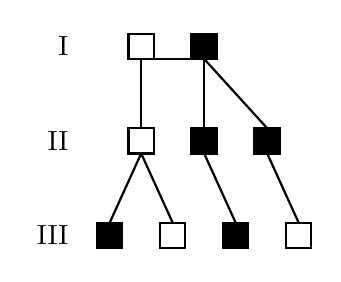
\begin{tikzpicture}[scale=0.8]
    % 第一代
    \draw[thick] (0, 5) rectangle (0.4, 5.4);
    \filldraw[thick, fill=black] (1, 5) rectangle (1.4, 5.4);
    \draw[thick] (0.2, 5) -- (1.2, 5);
    
    % 第二代
    \draw[thick] (0, 3.5) rectangle (0.4, 3.9);
    \filldraw[thick, fill=black] (1, 3.5) rectangle (1.4, 3.9);
    \filldraw[thick, fill=black] (2, 3.5) rectangle (2.4, 3.9);
    \draw[thick] (0.2, 5) -- (0.2, 3.9);
    \draw[thick] (1.2, 5) -- (1.2, 3.9);
    \draw[thick] (1.2, 5) -- (2.2, 3.9);
    
    % 第三代
    \filldraw[thick, fill=black] (-0.5, 2) rectangle (-0.1, 2.4);
    \draw[thick] (0.5, 2) rectangle (0.9, 2.4);
    \filldraw[thick, fill=black] (1.5, 2) rectangle (1.9, 2.4);
    \draw[thick] (2.5, 2) rectangle (2.9, 2.4);
    \draw[thick] (0.2, 3.5) -- (-0.3, 2.4);
    \draw[thick] (0.2, 3.5) -- (0.7, 2.4);
    \draw[thick] (1.2, 3.5) -- (1.7, 2.4);
    \draw[thick] (2.2, 3.5) -- (2.7, 2.4);
    
    % 标注
    \node[left] at (-0.8, 5.2) {I};
    \node[left] at (-0.8, 3.7) {II};
    \node[left] at (-0.8, 2.2) {III};
\end{tikzpicture}
\captionof{figure}{系谱图分析示例}
\end{center}

\textbf{分析步骤}:

\textbf{步骤 1}:判断显隐性
\begin{itemize}[leftmargin=2em]
    \item II-1 和 II-2 都正常,但 III-1 患病
    \item 说明是隐性遗传(无中生有)
\end{itemize}

\textbf{步骤 2}:判断常染色体还是性染色体
\begin{itemize}[leftmargin=2em]
    \item 如果是 $X$ 连锁隐性,II-1 正常,III-1 不应该患病
    \item 但 III-1 是男性患者,说明可能是常染色体隐性
    \item 如果是 $X$ 连锁隐性,II-2 应该是携带者,但 III-2 正常,不符合
    \item 因此判断为常染色体隐性遗传
\end{itemize}

\textbf{步骤 3}:确定基因型
\begin{itemize}[leftmargin=2em]
    \item I-1: $AA$(正常)
    \item I-2: $aa$(患病)
    \item II-1: $Aa$(正常,携带者)
    \item II-2: $Aa$(正常,携带者)
    \item III-1: $aa$(患病)
    \item III-2: $AA$ 或 $Aa$(正常)
\end{itemize}

\textbf{结果}:该遗传病为常染色体隐性遗传。
\end{examplebox}

\begin{lemmabox}{系谱图判断技巧}
\begin{itemize}[leftmargin=2em]
    \item \textbf{无中生有为隐性}:父母都正常,子代患病
    \item \textbf{有中生无为显性}:父母都患病,子代正常
    \item \textbf{隐性看女病}:隐性遗传时,看女性患者的父、子
    \item \textbf{显性看男病}:显性遗传时,看男性患者的母、女
    \item \textbf{伴性遗传特点}:与性别相关,交叉遗传
\end{itemize}
\end{lemmabox}

\subsection{概率计算}

\begin{examplebox}{系谱图概率计算}
\textbf{题目}:上例中,III-2 与一个正常女性(人群中携带者概率为 $\frac{1}{100}$)婚配,求子代患病的概率。

\textbf{解题}:

III-2 的基因型:$AA$ 或 $Aa$

III-2 是 $Aa$ 的概率 = $\frac{2}{3}$(因为 III-2 正常,排除 $aa$)

正常女性是 $Aa$ 的概率 = $\frac{1}{100}$

子代患病($aa$)的条件:
\begin{itemize}[leftmargin=2em]
    \item III-2 是 $Aa$(概率 $\frac{2}{3}$)
    \item 正常女性是 $Aa$(概率 $\frac{1}{100}$)
    \item 两者都是 $Aa$ 时,子代 $aa$ 的概率 = $\frac{1}{4}$
\end{itemize}

子代患病概率 = $\frac{2}{3} \times \frac{1}{100} \times \frac{1}{4} = \frac{1}{600}$

\textbf{结果}:子代患病概率为 $\frac{1}{600}$。
\end{examplebox}

% ============================================
% 第九部分:育种应用
% ============================================

\section{第九部分:育种应用}

\subsection{单倍体育种}

\begin{definitionbox}{单倍体育种}
\textbf{单倍体育种}:通过花药(花粉)离体培养获得单倍体植株,然后通过染色体加倍获得纯合子,从而缩短育种年限的方法。

\textbf{优点}:
\begin{itemize}[leftmargin=2em]
    \item 快速获得纯合子,缩短育种年限
    \item 后代不发生性状分离
    \item 可用于筛选优良性状
\end{itemize}
\end{definitionbox}

\begin{examplebox}{单倍体育种过程}
\textbf{过程}:

\textbf{步骤 1}:花药离体培养
\begin{itemize}[leftmargin=2em]
    \item 取 $F_1$ 的花药($AaBb$)
    \item 花药中的花粉是单倍体($AB$、$Ab$、$aB$、$ab$)
    \item 通过组织培养获得单倍体植株
\end{itemize}

\textbf{步骤 2}:染色体加倍
\begin{itemize}[leftmargin=2em]
    \item 使用秋水仙素处理单倍体植株
    \item 抑制纺锤体形成,使染色体加倍
    \item 获得纯合二倍体($AABB$、$AAbb$、$aaBB$、$aabb$)
\end{itemize}

\textbf{步骤 3}:筛选
\begin{itemize}[leftmargin=2em]
    \item 选择具有优良性状的纯合子
    \item 直接用于生产,不发生性状分离
\end{itemize}

\begin{center}
\begin{tikzpicture}[scale=0.8]
    % F1
    \node[rectangle, draw=myblue, thick, minimum width=2cm, minimum height=0.8cm] (F1) at (0, 4) {$F_1: AaBb$};
    
    % 花药
    \node[circle, draw=mygreen, thick, minimum size=0.6cm] (p1) at (-1.5, 2.5) {$AB$};
    \node[circle, draw=mygreen, thick, minimum size=0.6cm] (p2) at (-0.5, 2.5) {$Ab$};
    \node[circle, draw=mygreen, thick, minimum size=0.6cm] (p3) at (0.5, 2.5) {$aB$};
    \node[circle, draw=mygreen, thick, minimum size=0.6cm] (p4) at (1.5, 2.5) {$ab$};
    \draw[->, mygreen] (F1) -- (p1);
    \draw[->, mygreen] (F1) -- (p2);
    \draw[->, mygreen] (F1) -- (p3);
    \draw[->, mygreen] (F1) -- (p4);
    \node[below=0.1cm of p2, font=\tiny] {花药离体培养};
    
    % 单倍体
    \node[rectangle, draw=myorange, thick, minimum width=1cm, minimum height=0.5cm] (h1) at (-1.5, 1) {$AB$};
    \node[rectangle, draw=myorange, thick, minimum width=1cm, minimum height=0.5cm] (h2) at (-0.5, 1) {$Ab$};
    \node[rectangle, draw=myorange, thick, minimum width=1cm, minimum height=0.5cm] (h3) at (0.5, 1) {$aB$};
    \node[rectangle, draw=myorange, thick, minimum width=1cm, minimum height=0.5cm] (h4) at (1.5, 1) {$ab$};
    \draw[->, mypurple] (p1) -- (h1);
    \draw[->, mypurple] (p2) -- (h2);
    \draw[->, mypurple] (p3) -- (h3);
    \draw[->, mypurple] (p4) -- (h4);
    \node[below=0.1cm of h2, font=\tiny] {单倍体植株};
    
    % 纯合子
    \node[rectangle, draw=myred, thick, minimum width=1.2cm, minimum height=0.6cm] (d1) at (-1.5, -0.5) {$AABB$};
    \node[rectangle, draw=myred, thick, minimum width=1.2cm, minimum height=0.6cm] (d2) at (-0.5, -0.5) {$AAbb$};
    \node[rectangle, draw=myred, thick, minimum width=1.2cm, minimum height=0.6cm] (d3) at (0.5, -0.5) {$aaBB$};
    \node[rectangle, draw=myred, thick, minimum width=1.2cm, minimum height=0.6cm] (d4) at (1.5, -0.5) {$aabb$};
    \draw[->, mypurple] (h1) -- (d1);
    \draw[->, mypurple] (h2) -- (d2);
    \draw[->, mypurple] (h3) -- (d3);
    \draw[->, mypurple] (h4) -- (d4);
    \node[below=0.1cm of d2, font=\tiny] {染色体加倍};
    \node[below=0.5cm of d2, font=\small] {纯合二倍体};
\end{tikzpicture}
\captionof{figure}{单倍体育种过程}
\end{center}
\end{examplebox}

\subsection{无籽西瓜(三倍体)}

\begin{definitionbox}{三倍体}
\textbf{三倍体}:体细胞中含有三套染色体组的个体,染色体数为 $3n$。

\textbf{特点}:
\begin{itemize}[leftmargin=2em]
    \item 减数分裂时染色体不能正常配对
    \item 产生的配子大多不正常
    \item 无法形成正常的种子
    \item 应用:无籽西瓜、无籽香蕉
\end{itemize}
\end{definitionbox}

\begin{examplebox}{无籽西瓜的培育}
\textbf{原理}:三倍体西瓜在减数分裂时,同源染色体不能正常配对,导致配子染色体数异常,无法形成正常的种子。

\textbf{培育过程}:

\textbf{步骤 1}:获得四倍体
\begin{itemize}[leftmargin=2em]
    \item 用秋水仙素处理二倍体西瓜($2n = 22$)
    \item 染色体加倍,获得四倍体($4n = 44$)
\end{itemize}

\textbf{步骤 2}:获得三倍体
\begin{itemize}[leftmargin=2em]
    \item 四倍体($4n$)$\times$ 二倍体($2n$)
    \item 子代为三倍体($3n = 33$)
\end{itemize}

\textbf{步骤 3}:产生无籽西瓜
\begin{itemize}[leftmargin=2em]
    \item 三倍体植株开花
    \item 用二倍体花粉刺激(提供生长素)
    \item 果实发育,但种子不发育(无籽)
\end{itemize}

\begin{center}
\begin{tikzpicture}[scale=0.75]
    % 二倍体
    \node[rectangle, draw=myblue, thick, minimum width=1.5cm, minimum height=0.8cm] (2n) at (0, 4) {$2n = 22$};
    \node[below=0.2cm of 2n] {二倍体};
    
    % 秋水仙素处理
    \node[rectangle, draw=mygreen, thick, minimum width=1.5cm, minimum height=0.8cm] (4n) at (0, 2.5) {$4n = 44$};
    \node[below=0.2cm of 4n] {四倍体};
    \draw[->, myorange] (2n) -- (4n);
    \node[right=0.3cm of 4n, font=\tiny] {秋水仙素};
    
    % 三倍体
    \node[rectangle, draw=myred, thick, minimum width=1.5cm, minimum height=0.8cm] (3n) at (0, 1) {$3n = 33$};
    \node[below=0.2cm of 3n] {三倍体};
    \draw[->, mypurple] (4n) -- (3n);
    \node[left=0.3cm of 3n, font=\tiny] {$4n \times 2n$};
    
    % 减数分裂
    \node[rectangle, draw=mygray, thick, minimum width=2cm, minimum height=0.6cm] (meiosis) at (-2, -0.5) {减数分裂};
    \node[rectangle, draw=mygray, thick, minimum width=2cm, minimum height=0.6cm] (gamete) at (2, -0.5) {配子异常};
    \draw[->, mypurple] (3n) -- (meiosis);
    \draw[->, mypurple] (meiosis) -- (gamete);
    
    % 无籽
    \node[rectangle, draw=myorange, thick, minimum width=2cm, minimum height=0.6cm] (seedless) at (0, -1.5) {无籽西瓜};
    \draw[->, mypurple] (gamete) -- (seedless);
\end{tikzpicture}
\captionof{figure}{无籽西瓜培育过程}
\end{center}
\end{examplebox}

\begin{lemmabox}{三倍体无籽的原理}
\begin{itemize}[leftmargin=2em]
    \item \textbf{减数分裂异常}:三倍体减数分裂时,同源染色体不能正常配对
    \item \textbf{配子异常}:产生的配子染色体数大多不正常($n$、$2n$、$0$ 等)
    \item \textbf{无法受精}:异常配子无法正常受精,不能形成种子
    \item \textbf{需要刺激}:用二倍体花粉刺激,提供生长素,使果实发育
    \item \textbf{应用}:无籽西瓜、无籽香蕉、无籽柑橘
\end{itemize}
\end{lemmabox}

% ============================================
% 第十部分:解题技巧总结(原第六部分)
% ============================================

\section{第十部分:解题技巧总结与快速参考}

\subsection{配子法解题流程}

\begin{lemmabox}{配子法标准流程}
\begin{enumerate}[leftmargin=2em]
    \item \textbf{确定亲本基因型}
        \begin{itemize}
            \item 直接给出
            \item 通过表现型推断
            \item 通过子代逆推
        \end{itemize}
    \item \textbf{分析配子类型及比例}
        \begin{itemize}
            \item 每对基因独立分离
            \item 多对基因自由组合
            \item 注意纯合子只产生一种配子
        \end{itemize}
    \item \textbf{计算配子结合概率}
        \begin{itemize}
            \item 使用棋盘格(直观)
            \item 使用概率乘法(快捷)
        \end{itemize}
    \item \textbf{统计子代结果}
        \begin{itemize}
            \item 合并相同基因型
            \item 根据显隐性确定表现型
            \item 计算比例或概率
        \end{itemize}
\end{enumerate}
\end{lemmabox}

\subsection{常见比例及对应基因型}

\begin{lemmabox}{经典分离比}
\begin{itemize}[leftmargin=2em]
    \item \textbf{$3:1$}:$Aa \times Aa$(完全显性,$F_2$)
    \item \textbf{$1:1$}:$Aa \times aa$(测交)
    \item \textbf{$1:2:1$}:$Aa \times Aa$(不完全显性,$F_2$)
    \item \textbf{$9:3:3:1$}:$AaBb \times AaBb$(两对独立基因,$F_2$)
    \item \textbf{$1:1:1:1$}:$AaBb \times aabb$(测交)
    \item \textbf{$3:3:1:1$}:$AaBb \times Aabb$ 或 $AaBb \times aaBb$
    \item \textbf{$27:9:9:9:3:3:3:1$}:$AaBbCc \times AaBbCc$(三对独立基因,$F_2$)
    \item \textbf{$9:7$}:互补作用(基因互作)
    \item \textbf{$9:6:1$}:累加作用(基因互作)
    \item \textbf{$12:3:1$}:显性上位(基因互作)
    \item \textbf{$9:3:4$}:隐性上位(基因互作)
    \item \textbf{$13:3$}:抑制作用(基因互作)
    \item \textbf{$2:1$}:显性致死或隐性致死
\end{itemize}
\end{lemmabox}

\subsection{快速计算方法}

\begin{examplebox}{分离定律快速计算}
对于独立遗传的多对基因,可以分别计算每对基因,然后相乘。

\textbf{公式}:
\begin{itemize}[leftmargin=2em]
    \item 子代基因型种类 = $\prod_{i=1}^{n} m_i$($m_i$ 为第 $i$ 对基因的子代基因型种类)
    \item 子代表现型种类 = $\prod_{i=1}^{n} p_i$($p_i$ 为第 $i$ 对基因的子代表现型种类)
    \item 特定基因型概率 = $\prod_{i=1}^{n} P_i$($P_i$ 为第 $i$ 对基因的相应基因型概率)
\end{itemize}

\textbf{例子}:$AaBbCc \times AabbCc$

第一对 ($Aa \times Aa$):$AA$ ($\frac{1}{4}$)、$Aa$ ($\frac{1}{2}$)、$aa$ ($\frac{1}{4}$)

第二对 ($Bb \times bb$):$Bb$ ($\frac{1}{2}$)、$bb$ ($\frac{1}{2}$)

第三对 ($Cc \times Cc$):$CC$ ($\frac{1}{4}$)、$Cc$ ($\frac{1}{2}$)、$cc$ ($\frac{1}{4}$)

子代 $AabbCc$ 的概率 = $\frac{1}{2} \times \frac{1}{2} \times \frac{1}{2} = \frac{1}{8}$
\end{examplebox}

\subsection{易错点提醒}

\begin{notebox}{常见错误}
\begin{enumerate}[leftmargin=2em]
    \item \textbf{配子类型遗漏}:多对基因时,注意配子种类数 = $2^n$($n$ 为杂合对数)
    \item \textbf{比例计算错误}:合并相同基因型时,概率要相加
    \item \textbf{显隐性判断}:注意不完全显性、共显性等特殊情况
    \item \textbf{独立遗传假设}:确认基因是否位于非同源染色体上
    \item \textbf{条件概率}:注意题目问的是"在...中"的条件概率
    \item \textbf{致死基因}:考虑致死基因型后,要重新计算比例
    \item \textbf{连锁遗传}:注意区分连锁遗传和独立遗传,互换概率的范围
    \item \textbf{伴性遗传}:注意性染色体的遗传方式,正反交结果不同
    \item \textbf{基因互作}:注意表现型比例偏离 $9:3:3:1$ 的情况
    \item \textbf{系谱图分析}:注意判断显隐性和常染色体/性染色体
    \item \textbf{三倍体}:注意三倍体减数分裂异常,配子大多不正常
    \item \textbf{母本效应}:注意正反交结果不同,子代表现型由母本决定
\end{enumerate}
\end{notebox}

% ============================================
% 附录:公式速查表
% ============================================

\section{附录:公式速查表}

\subsection{配子种类计算公式}

\begin{lemmabox}{配子种类数}
\begin{itemize}[leftmargin=2em]
    \item 一对等位基因:$Aa$ 产生 $2$ 种配子
    \item $n$ 对独立等位基因:产生 $2^n$ 种配子
    \item 杂合对数 $m$:产生 $2^m$ 种配子
    \item 纯合子:只产生 $1$ 种配子
\end{itemize}
\end{lemmabox}

\subsection{子代基因型和表现型种类}

\begin{lemmabox}{种类数计算}
\begin{itemize}[leftmargin=2em]
    \item \textbf{基因型种类}:
        \begin{itemize}
            \item 一对基因:$3$ 种($AA$、$Aa$、$aa$)
            \item $n$ 对独立基因:$3^n$ 种
        \end{itemize}
    \item \textbf{表现型种类}(完全显性):
        \begin{itemize}
            \item 一对基因:$2$ 种
            \item $n$ 对独立基因:$2^n$ 种
        \end{itemize}
    \item \textbf{表现型种类}(不完全显性):
        \begin{itemize}
            \item 一对基因:$3$ 种
            \item $n$ 对独立基因:$3^n$ 种
        \end{itemize}
\end{itemize}
\end{lemmabox}

\subsection{概率计算技巧}

\begin{lemmabox}{概率计算}
\begin{itemize}[leftmargin=2em]
    \item \textbf{乘法原理}:独立事件同时发生的概率 = 各事件概率的乘积
    \item \textbf{加法原理}:互斥事件任一发生的概率 = 各事件概率的和
    \item \textbf{条件概率}:$P(A|B) = \frac{P(A \cap B)}{P(B)}$
    \item \textbf{至少一个}:$P(\text{至少一个}) = 1 - P(\text{全不})$
\end{itemize}
\end{lemmabox}

\subsection{三对等位基因计算公式}

\begin{lemmabox}{三对等位基因}
\begin{itemize}[leftmargin=2em]
    \item \textbf{配子种类}:$2^3 = 8$ 种
    \item \textbf{基因型种类}:$3^3 = 27$ 种
    \item \textbf{表现型种类}(完全显性):$2^3 = 8$ 种
    \item \textbf{表现型比例}:$(3:1)^3 = 27:9:9:9:3:3:3:1$
    \item \textbf{计算方法}:分离定律分别计算,然后用乘法原理组合
\end{itemize}
\end{lemmabox}

\subsection{连锁遗传计算公式}

\begin{lemmabox}{连锁遗传}
\begin{itemize}[leftmargin=2em]
    \item \textbf{互换概率}(测交法):$r = \frac{\text{重组型个体数}}{\text{总个体数}} \times 100\%$
    \item \textbf{互换概率}(自交法):$r = \frac{\text{重组型个体比例}}{1} \times 100\%$
    \item \textbf{重组型配子比例}:$\frac{r}{2}$
    \item \textbf{亲本型配子比例}:$\frac{1-r}{2}$(每种)
    \item \textbf{范围}:$0\% \leq r \leq 50\%$
    \item \textbf{完全连锁}:$r = 0\%$,只有亲本型配子
    \item \textbf{独立遗传}:$r = 50\%$,等于自由组合
\end{itemize}
\end{lemmabox}

\subsection{伴性遗传计算公式}

\begin{lemmabox}{伴性遗传}
\begin{itemize}[leftmargin=2em]
    \item \textbf{X 连锁隐性}:男性患者比例 = 基因频率
    \item \textbf{X 连锁显性}:女性患者多于男性患者
    \item \textbf{Y 连锁}:只在男性中遗传,父传子
    \item \textbf{交叉遗传}:男性患者 $\to$ 女儿(携带者)$\to$ 外孙(患者)
    \item \textbf{概率计算}:考虑性别比例,X 染色体随机分配
\end{itemize}
\end{lemmabox}

\subsection{基因互作比例}

\begin{lemmabox}{基因互作}
\begin{itemize}[leftmargin=2em]
    \item \textbf{互补作用}:$9:7$(需要两对显性基因)
    \item \textbf{累加作用}:$9:6:1$(显性基因数量决定)
    \item \textbf{显性上位}:$12:3:1$(一对基因抑制另一对)
    \item \textbf{隐性上位}:$9:3:4$(一对隐性基因抑制另一对)
    \item \textbf{抑制作用}:$13:3$(一对基因抑制另一对的表达)
    \item \textbf{基础比例}:独立遗传时为 $9:3:3:1$
\end{itemize}
\end{lemmabox}

\subsection{致死基因计算}

\begin{lemmabox}{致死基因}
\begin{itemize}[leftmargin=2em]
    \item \textbf{存活个体比例}:$1 - P(\text{致死基因型})$
    \item \textbf{调整后比例}:$\frac{P(\text{基因型})}{P(\text{存活})}$
    \item \textbf{显性致死}:显性纯合子或杂合子致死
    \item \textbf{隐性致死}:隐性纯合子致死
    \item \textbf{配子致死}:某些配子不能形成
    \item \textbf{合子致死}:某些合子不能发育
\end{itemize}
\end{lemmabox}

% ============================================
% 文档结束
% ============================================

\end{document}